%
% METU Institute of Natural and Applied Sciences Thesis example 
%
% Edited and Commented by Utku Erdoğdu 2013
%
% Please read the explanations so that you can customize the document		
%
% Files needed by this document:
% metu.cls 
% metu11.def (if you will use 11pt fonts) 
% metu12.def (if you will use 12pt fonts)
% metu10.def (if you will use 10pt fonts)
%
% Possible Options Here:
%
% oneandhalf, double, single : Line spacing used in the thesis. Default and institute preference is
% single.
%
% 10pt, 11pt, 12pt : Font size Default is 10pt, which is institue choice. 
% 
% pntr, pntc, pnbt : Page number position. Options are top center, top right or bottom. Default and
% institute preference is page numbers at bottom. When page numbers are at the top bottom margins
% are skewed.
% 
% chaproman, chaparabic: Chapter numbering format. Options are roman numbers and arabic numbers.
% Default is roman, institute prefers arabic
%
% oneside, twoside : Printing style. Default is twoside, which is institute choice. In this style
% chapters begin from odd numbered pages.
%
% tr, eng : Document language. This is useful if you want to translate your thesis into
% Turkish. Then you give the option tr and use \ifturkish. . .\else. . .\fi  whenever you want 
% to do something only for Turkish or only for English. Default is eng. 
% IMPORTANT!! : For official institute documents you should not use this option. 
% The Turkish format is only supplied for custom translations.
%
% ceng,aee,arme.. : You can use the abbreviated form of your department here and there is no further need to
% define the department name below. If your department name is not among the below list of defined
% departments, you should use \department and \turkishdepartment macros to define the name of your
% department.
%
% Defined Departments and Abbreviations:
% --------------------------------------
% Computer Engineering : ceng
% Aerospace Engineering : aee
% Archaeometry : arme
% Architecture : arch
% Biochemistry : bch
% Biology : biol
% Biomedical Engineering : bme
% Biotechnology : btec
% Building Science : bs
% Cement Engineering : ceme
% Chemical Engineering : che
% Chemistry : chem
% City and Regional Planning : crp
% City Planning : cp
% Civil Engineering : ce
% Computational Design and Fabrication Technologies in Architecture : arcd
% Computer Education and Instructional Technology : cte
% Design Research for Interaction : iddi
% Earthquake Studies : eqs
% Earth System Science : ess
% Electrical and Electronics Engineering : ee
% Engineering Management : em
% Engineering Sciences : es
% Environmental Engineering : enve
% Food Engineering : fde
% Geodetics - Geographical Information Technologies : ggit
% Geological Engineering : geoe
% Hydrosystems Engineering : he
% Industrial Design : id
% Industrial Engineering : ie
% Mathematics : math
% Mechanical Engineering : mech
% Metallurgical and Materials Engineering : mete
% Micro and Nanotechnology : mnt
% Mining Engineering : mine
% Operational Research : or
% Petroleum and Natural Gas Engineering : pete
% Physics : phys
% Polymer Science and Technology : pst
% Regional Planning : rp
% Restoration : rest
% Secondary Science and Mathematics Education : ssme
% Software Engineering : se
% Statistics : stat
% Structural Mechanics : st
% 
% phd, ms : Degree Received. Ph.D. or M.S. Default is M.S.
%
% End of Options
\documentclass[chaparabic,ceng,ms,12pt,oneandhalf]{metu}
% You can delete next line If your thesis does not have an appendix
\usepackage{appendix}

%
% Use your latex packages here
\usepackage{paralist}
\usepackage{amsthm}
\theoremstyle{definition}
\newtheorem{definition}{Definition}[section]
\usepackage{booktabs}
\usepackage{amssymb} 
\usepackage{subcaption}
\usepackage{url}
 
\usepackage[linesnumbered,ruled,vlined]{algorithm2e}

% End of Latex Packages
%
% Any personal Latex definition, decleration, etc.


% End of personal stuff
%
% Personal Information 
% ----------------------------
%
% Please check this part and fill in information about your thesis
%
% Name and Surname
\author{Onur Yılmaz}
% Thesis Title English and Turkish
\title{Recommendation Generation for Performance Improvement by using Cross-Organizational Process Mining}
\turkishtitle{Çapraz Organizasyon Süreç Madenciliği Kullanarak Performans Gelişimi için Öneri Üretimi}
% Department : English and Turkish
%
% Some of the departments are pre-defined, you need not redeclare them. You can use them by just
% giving an option to \documentclass. See documentation for options above. If you will define your 
% department here do not use ``Department'' or ``Bölümü'' words.
%\department{Computer Engineering}
%\turkishdepartment{Bilgisayar Mühendisliği}
%
%
% Date : You should indicate the month of your thesis defence in English.
% Default is this month
%
\date{September 2015}
%
% Approval Page Details
% --------------------------
% For each command you can give the title as optional parameter enclosed in [ ]
% This also handles the Turkish titles if you're planning to produce Turkish version of the
% document. If you'll hard code the title, you need to use turkish version of each command after
% the command itself
% 
% prof : Prof. Dr.
% assocprof : Assoc. Prof. Dr.
% assistprof : Assist. Prof. Dr.
% dr : Dr.
%
% Director of Institute
\director[prof]{Gülbin Dural Ünver}
% Head of Department
\headofdept[prof]{Adnan Yazıcı}
%
% Supervisor : English and Turkish
\supervisor[assocprof]{Pınar Karagöz}
% \turkishsupervisor{  } %if you will hard-code the academic title
%
% Affiliation of Supervisor in English and possibly in Turkish
\departmentofsupervisor{Computer Engineering Department, METU}
% Co Supervisor if Any : English and Turkish
% You can just delete the next line if you don't have a co-supervisor
%\cosupervisor[assocprof]{Bedir Tekinerdoğan}
% \turkishcosupervisor{Prof. Dr. Reda Alhajj} %if you will hard-code the academic title
% Affiliation of Co-Supervisor
% You can just delete the next line if you don't have a co-supervisor
%
% Committee Members
% In general members are sorted according to their academic titles
%
% Proffesors (1)
% Associate Professors (2)
% Assistant Professors (3)
% Other (4)
% 
% IMPORTANT:  All affiliatons should fit in a single line
% If affiliation line is broken into two lines you should shorten the affiliation by using 
% abbrevations or any other means
%
% First committee member should be the chair of examining committee
% Typically the chair is one of the highest ranked committee members
% Ask your supervisor if you are not sure
\committeememberi[assocprof]{Pınar Karagöz}
\affiliationi{Computer Engineering Department, METU}
% Second committee member is always your supervisor
\committeememberii[assocprof]{Pınar Karagöz}
\affiliationii{Computer Engineering Department, METU}
% If you are an M.Sc. student and your Co-Supervisor is in your 
% examination committee, then third committee member is always your co-supervisor
%
% IMPORTANT: If you are Ph.D. student your co-supervisor can not be in your 
% examination committee.
\committeememberiii[assocprof]{Pınar Karagöz}
\affiliationiii{Computer Engineering Department, METU}
% Fourth committee member
\committeememberiv[assocprof]{Pınar Karagöz}
\affiliationiv{Computer Engineering Department, METU}
% Fifth committee member
\committeememberv[assocprof]{Pınar Karagöz}
\affiliationv{Computer Engineering Department, METU}
%
% Keywords : English & Turkish, Comma seperated
\keywords{Process Mining, Cross-organizational Process Mining, Recommendation Generation, Process Performance Improvement}
\anahtarklm{Süreç Madenciliği, Çapraz Organizasyon Süreç Madenciliği, Öneri Geliştirme, Süreç Performans İyileştirme}
%
% Abstract in English
% at most 250 words
\abstract{Process mining is a relatively young and developing research area with the main idea of discovering, monitoring and improving processes by extracting information from the event logs. With the increase of cloud computing and shared infrastructures, event logs of multiple organizations are available for analysis where cross-organizational process mining stands with the opportunity for organizations learning from each other. Approach proposed in this study mines process models of organizations and calculates performance indicators; followed by clustering of organizations based on performance indicators and finally spots mismatches between the process models to generate recommendations. This approach is implemented as extensible and configurable plugin set in ProM framework and tested for both synthetic and real life logs for efficiency of each stage with successful and suitable results within evaluation metrics. Generated recommendation results indicate that using this approach to generate recommendations significantly helps users to focus on areas of organizations process models for potential performance improvement which are difficult to spot manually and visually.}
%
% Turkish Abstract
%
\oz{Süreç madenciliği nispeten genç ve gelişmekte bir araştırma alanı olarak, olay günlüklerinden bilgi çıkartarak süreçlerin keşfedilmesi, iyileştirilmesi ve izlenmesini amaçlar. Bulut teknolojileri ve paylaşılan altyapıların yükselen kullanımı, birden çok organizasyona ait olay günlüklerini analiz etme imkanı sağlarken, çapraz organizasyon süreç madenciliği, organizasyonların birbirlerinden öğrenme imkanı yaratmasıyla öne çıkmaktadır. Bu tez çalışmasında önerilen yaklaşım, farklı organizasyonların süreç modellerini keşfetmekte ve performans göstergelerini hesaplamaktadır; organizasyonlar performans göstergelerine dayanarak kümelenmekte ve öneriler geliştirmek için organizasyonların süreç modelleri arasındaki uyumsuzluklar ortaya çıkarılmaktadır. Çalışmada önerilen yöntem, ProM uygulama çerçevesinde genişletilebilir ve yapılandırılabilir eklenti paketi olarak geliştirilmiş ve her aşaması sentetik ve gerçek hayat olay günlükleri ile test edilmiştir. Değerlendirme ölçütleri dahilinde başarılı ve uygun olan yöntem sonucu geliştirilen önerilerin, kullanıcıların manuel olarak fark etmesinin zor olduğu potansiyel performans iyileştirilmesi içeren süreç modeli kısımlarına odaklanmasına önemli ölçüde yardımcı olduğu gösterilmektedir.} 
%
% Dedication 
\dedication{\textit{To my family}}
%
%
% Acknowledgements   
\acknowledgments{
I would like to express my deepest gratitude to my advisor, Assoc. Prof. Pınar Karagöz, for her excellent guidance, support, patience, and positive attitude during my thesis studies.

I am also very grateful and would like to thank my family for their support, love and encouragement during my everlasting educational life.
}
%
% End of Personal and Introductory Information
%%%%%%%%%%%%%%%%%%%%%%%%%%%%%%%%%5

%%% !!! This two should be last lines before \begin{document}, do no move them !!!
\usepackage[pdftex]{hyperref}
\usepackage[all]{hypcap}
\usepackage{todonotes}
\usepackage{graphicx}
\graphicspath{ {./images/} }
\usepackage{rotating}
\usepackage{xy} 
\usepackage{booktabs}
\usepackage{pifont}
\usepackage{color}
\usepackage{listings}
\usepackage{pdfpages}
\usepackage{array}
\newcolumntype{M}{>{\centering\arraybackslash}m{\dimexpr.25\linewidth-2\tabcolsep}}
\renewcommand\lstlistingname{XChor Language - }
\def\lstlistingautorefname{XChorCode.}
\lstset{
language = java,
basicstyle=\small,
numbers=left,
numbersep=10pt,
numberstyle=\tiny\color{black},
stepnumber=1,
tabsize=2,
showspaces=false, 
frame=single,
breaklines=true,
escapeinside=~~
}
\usepackage{float}
\restylefloat{figure}
\newcommand{\tab}{\hspace*{2em}}
\DeclareGraphicsExtensions{.pdf,.png,.jpg}

\begin{document}
% Preliminaries
\begin{preliminaries}
% If you are willing to use any custom stuff before Chapters, put it here
% Such as List of Abbreviations
% Check the abbreviations.tex for a template list of abbreviations

\begin{theglossary}{LONGESTABBRV}
\item[BPM] Business Process Management
\item[BPMN] Business Process Modeling Notation
\item[CoSeLoG] Configurable Services for Local Governments
\item[ERP] Enterprise Resource Planning
\item[OMG] Object Management Group
\item[ProM] Process Mining Framework
\item[SBPMI] Shared Business Process Management Infrastructure
\item[WEKA] Waikato Environment for Knowledge Analysis
\end{theglossary}

% End of Preliminaries
\end{preliminaries}
%   
% Latex content Goes Here 
% 
%

% CHAPTER 1

\chapter{INTRODUCTION}
\label{chp:introduction}

Introduction goes here... 


\chapter{RELATED WORK}
\label{chp:relatedwork}

In this chapter, studies related to the work presented in this thesis are summarized. Firstly, latest trends and studies in the process mining area are explained. Then studies from cross-organizational process mining, which is the main topic of this research, is introduced. Following these, studies related to similarity in process mining is mentioned. Finally, performance and conformance analysis approaches in process mining area are presented.

\section{State of the Art in Process Mining}
\label{sec:state-of-the-art-in-process-mining}

In this section, important milestones in process mining and current research trends will be presented. Studies in process mining area have roots based on process discovery techniques for software engineering. These original techniques are studied to discover workflows using neural networks, finite state machines and Markovian approaches \cite{van2004process}. However, using process mining in the workflow management area is introduced by Agrawal et al. and this study aims to find workflow graphs given event logs and identify edge conditions between nodes \cite{agrawal1998mining}. In the following efforts, various different approaches based on hierarchical structuring, dependency and frequency graphs; and heuristic methods are suggested to address the same problem. While some of these algorithms are focused on creating partial solutions, some of the algorithms are used as a foundation for further expansions such as "Alpha Algorithm" of van der Aalst et al.\cite{van2004workflow}. Spread of process mining is not only in kept in academia, but also many vendors presented tools and software to discover processes and help organizations manage their workflows \cite{accorsi2014unleashing}.

\begin{figure}
  \centering
  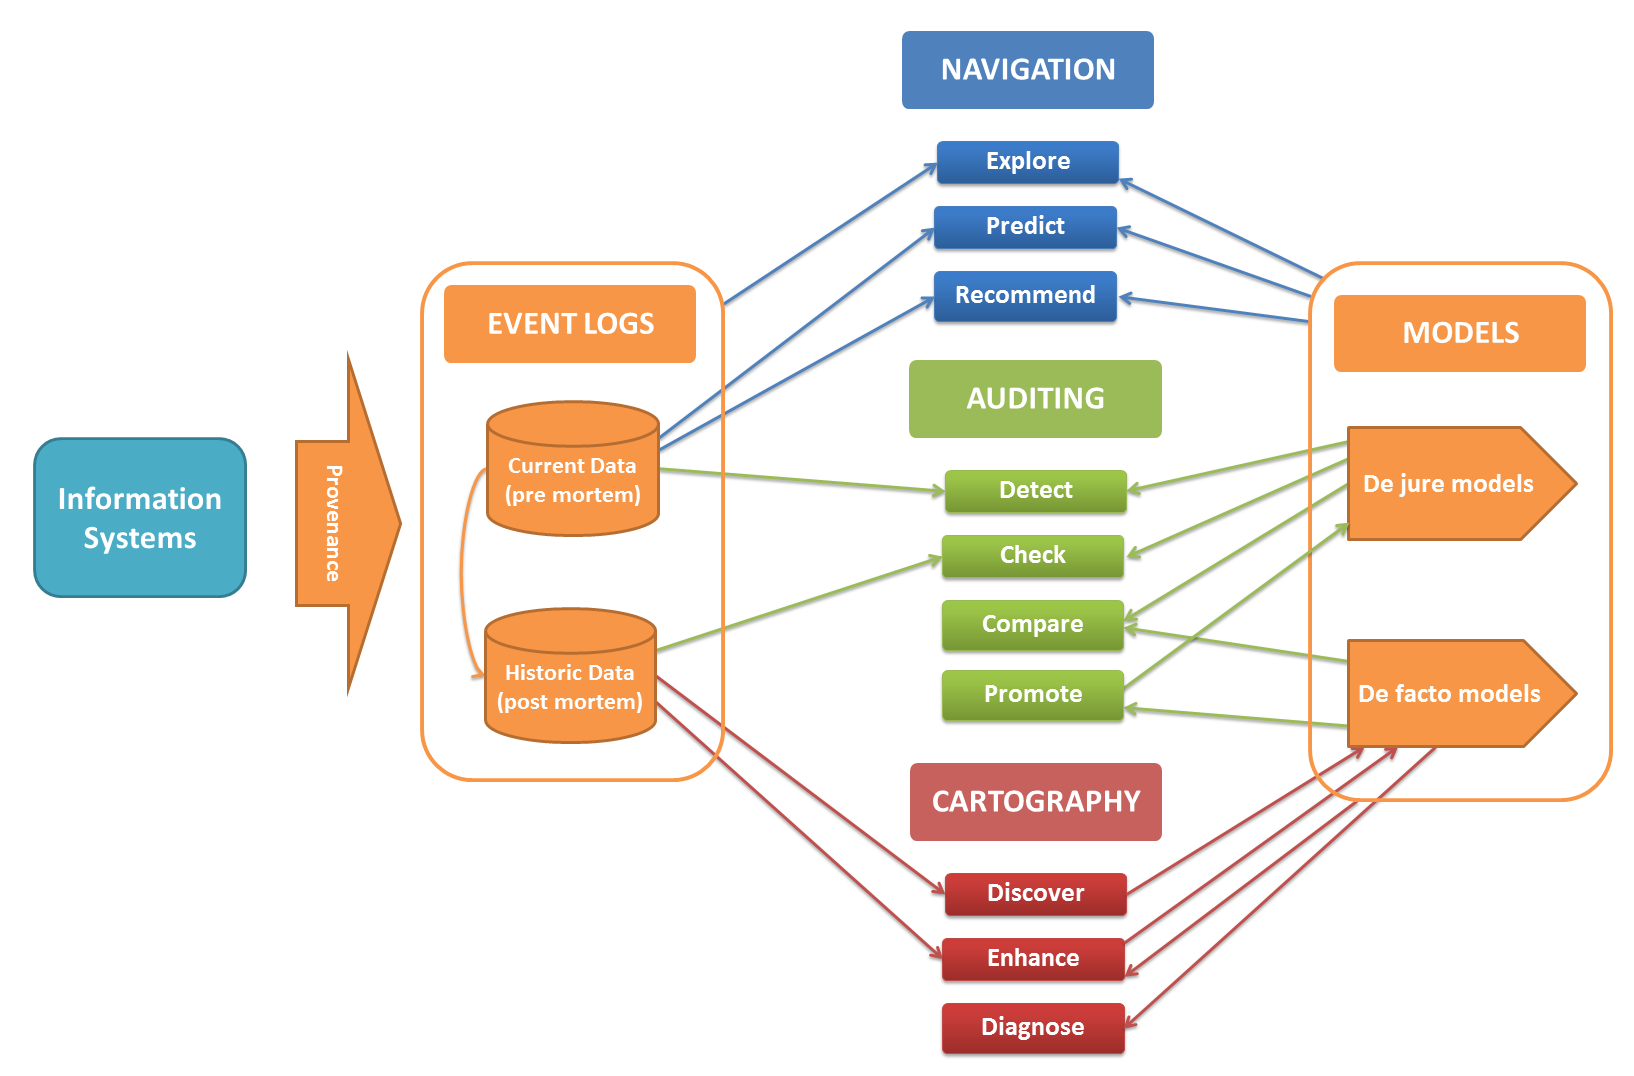
\includegraphics[width=\textwidth]{2_relatedwork/process-mining-spectrum-v2}
  \caption{Process Mining Framework}
  \label{fig:process-mining-spectrum-v2}
\end{figure}

Current challenges in the process mining area can be presented best through mentioning spectrum and its relations. As diagrammed in Figure~\ref{fig:process-mining-spectrum-v2} and presented in the research of van der Aalst \cite{van2011process}, process mining spectrum is extensive and highly inter-related. Starting with the provenance, process mining deals with gathering and keeping event logs as \textit{current data} and \textit{historic data}. In this level, \textit{post mortem data} means the logs and information gathered from completed events whereas \textit{pre mortem data} means information related to ongoing cases. This separation helps us to use historical knowledge to exploit and gain advantage over current business operations. At the right end of the diagram, models are presented as \textit{de facto models} and \textit{de jure models}. \textit{De jure models} are created with the aim of describing reality as it should be whereas \textit{de facto models} aims to describe reality as it is. Within each model category a mixture of perspectives, in other words point of views from different information levels, can be mixed. In order to fill the gap between event logs and models, ten different process mining activities are listed under three categories \cite{van2011process} as follows:
\begin{description}
\item[Cartography:] In this category the main aim is to create maps of the real world activities by using process models. 
	\begin{description}
	\item[Discovery:] Discovery is focused on extracting process models from event logs. 
	\item[Enhancing:] Enhancing activities are based on improving \textit{de facto models} with the information hidden in the event logs. 
	\item[Diagnose:] Diagnose activities stand for identifying the problems caused by directly process models.
	\end{description}
\item[Auditing:] In this category, activities related to confronting the model and the reality are collected.
	\begin{description}
	\item[Detect:] Detection is based on comparing the \textit{de jure models} with the ongoing processes to generate alerts if shifts occur in the reality.
	\item[Check:] Checking is defined to identify deviations occurred in the past.
	\item[Compare:] Comparison of \textit{de facto models} and \textit{de jure models} shows the difference between planned and the reality.
	\item[Promote:] Promotion includes  partially updating \textit{de jure models} from the information gathered from \textit{de facto models}.
	\end{description}
\item[Navigation:] In this category, process mining methods are used like a navigation application.
	\begin{description}
	\item[Explore:] Event data and models are used in combination to explore business processes.
	\item[Predict:] Prediction activities combine the information from past events and make predictions about ongoing processes.
	\item[Recommend:] Suitable actions can be suggested by using the prediction and contextual  information.
	\end{description}
\end{description}

Within this framework, the study presented in this thesis is a combination of discovery from cartography, promoting from auditing and recommendation from navigation. In other words and within the metaphor of spectrum, this study aims to discover maps using the discovery techniques and promotes the partially best locations in the map to create recommendations for travelers in their navigation applications. 

\section{Process Discovery in Process Mining}
\label{sec:process-discovery-in-process-mining} 
In this section, process discovery studies will be presented briefly. Within the process mining framework, there are various different process mining algorithms proposed which have the same aim of discovering underlying processes. Considering the approaches undertaken with the proposed algorithms, the following grouping is provided \cite{khodabandelou2013process}.
\begin{description}
\item[$\alpha$-algorithm:] This algorithm is based on the causality relationship that can be discovered from the event logs and proposed by van der Aalst et al. \cite{van2004workflow}. However, this approach cannot handle loops and therefore extensions like $\alpha$++ algorithm \cite{de2004process} is proposed to overcome this problem. Outputs of this approach and its extensions are workflow nets with XOR, AND splits and joins to represent underlying process models.
\item[Inductive Approach:] Methods proposed in inductive approach \cite{herbst1998integrating, herbst2000dealing} are based on finding the best Hidden Markov Models (HMMs) that represents the underlying process model. Workflow nets are constructed by using HMM nodes and inductive learning.
\item[Hierarchical Clustering:] This method \cite{greco2005mining} firstly splits the event logs into clusters and creates a dependency graph. Using this dependency graph, clusters are defined with a hierarchy tree which is then merged into a single workflow model.
\item[Genetic Approach:] The first method provided in this group \cite{van2005genetic} constructs models based on causal matrix of activities and tries to handle noise, incompleteness, concurrency, hidden and duplicate activities. However, there are many configuration parameters and fine-tuning to handle noise and irrelevant data to use this method. Second method in this group \cite{esgin2010hybrid} applies genetic algorithms to discover process models using from-to charts and this method finds optimal or sub-optimal solutions for a relatively complex processes within a reasonable processing time.
\item[Heuristic Approach:]Heuristic approach for process discovery is an extension of $\alpha$-algorithm which is based on likelihood calculation of activities and constructs dependency and frequency graphs while handling the noise in the event log. In addition, heuristic approach is used to locate the immediate successors with the help of evaluation metrics generated over raw from-to charts \cite{esgin2009hybrid}.
\end{description}
 
Proposed methods in process discovery are based on solving different challenges in the process mining area. Considering the scope of this thesis study; process discovery operations are undertaken with inductive methods which is a robust, repeatable and mature set of approaches.

\section{Cross-organizational Process Mining}
\label{sec:cross-organizational-process-mining}
In this section, related studies and trends in cross-organizational process mining will be presented. Cross-organizational mining is based on cross-correlation of workflows and the realized activities in different organizations. The main challenge of this topic in process mining is that comparing processes and their performances of different organizational units in an objective approach. This objective approach is open to be enhanced with the process context, namely the environment of the process that is executed. Most of the studies in this area are currently studying to reveal the possible opportunities and some initial approaches to address main challenges.

In the study of Bujis et al. \cite{buijs2012towards}, the authors indicated the importance of the increase of Software-as-a-Service (SaaS) and cloud computing infrastructure usages. As a result of this increase, more and more organizations will use a Shared Business Process Management Infrastructure (SBPMI) and it is an opportunity for different organizational units to learn from each other in such infrastructure. The approach presented in this study is based on three questions and three metric groups to answer these questions:
\begin{enumerate}
\item Which organizations support my behavior with better process models?
\item Which organizations have better behavior which my process model supports? and
\item Which set of organizations can I support with my process model?
\end{enumerate} While answering these questions, they used \textit{simplification based metrics} to indicate better process models; and \textit{throughput time metrics} to indicate better behaviors. In this study, it is shown how a generic framework can be used to highlight the main idea behind cross-organizational process mining. 

In the study of van der Aalst \cite{van2011business}, using configurable process models is proposed for the organizations sharing the same infrastructure and doing the similar work. Configurable process models are defined as a family of process models where each organization can use this family with their configurations according to their business needs. This approach not only creates behaviors needed by each organization but also creates a basis to compare and learn within process mining framework. The configurable process models are formalized by "Causal Nets", which is a notational language based on input and output bindings of each node. Although this study does not provide answer to all challenges related to cross-organizational-process-mining, a formalism of configurable processes models is presented to address learning and conformance checking.

Cross-organizational process mining is divided into intra-organizational and inter-organizational process mining subcategories with two basic ideas: \textit{collaboration} and \textit{exploiting commonality} \cite{van2011intra}. In his study, van der Aalst defined \textit{collaboration} for distributed work between multiple organizations and \textit{commonality} as ability of using the same process models and infrastructure between the organizations. In order to exploit these two ideas, two partitioning dimensions are suggested in \cite{van2011intra}:
\begin{description}
\item[Vertical Partitioning:] Process instances, namely cases, distributed over several organizations which collaborate to complete a complex activity. 
\item[Horizontal Partitioning:] Process parts, namely tasks or activities, are shared within organizations like jigsaw puzzle parts.
\end{description}
For these orthogonal dimensions, a number of questions and challenges are presented in the study  \cite{van2011intra}. For the vertical partitioning, where organizations are aiming to share infrastructure and knowledge to learn from each other, it is mentioned that supervised learning methods like classification can be used. Notion of this thesis is based on vertical partitioning of cross-organizational process mining with the idea of unsupervised learning where predictor variables related to performances of organizations are used.
 
\section{Process Similarity in Process Mining}
\label{sec:process-similarity-in-process-mining}

In this section, prominent studies related to similarity in process mining will be presented with their results. With the emerging attention in business processes, organizations become aware of the fact that they can exploit the business processes and their similarities \cite{buijs2014comparing}. In addition, most of the large organizations have repository of process models of similar business operations \cite{dijkman2011similarity}. There are four main different approaches proposed to this solution in the literature currently. 

The first approach, proposed by Dijkman et al. \cite{dijkman2011similarity}, is based on similarity metrics as 
\begin{inparaenum}[\itshape a\upshape)]
\item node matching similarity;
\item structural similarity; and
\item behavioral similarity.
\end{inparaenum}
Result of the study \cite{dijkman2011similarity} indicates that using these three similarities can differentiate comparable process models and within these metrics structural similarity is the most prominent one. 

The second approach by Bujis and Reijis is an analytical approach \cite{buijs2014comparing} to compare the process models of different organizations that does similar works. Proposed algorithm is based on creating an alignment matrix between observed and realized models. This inter-relation is also used to compare different variants of the same process by different organizations. In addition, they suggested their method as a framework to further standardize a process of common interest. 

The third approach proposed by Esgin and Senkul focuses on delta analysis between predefined models and discovered models. In \cite{esgin2011delta}, a hybrid model which considers the dependencies of process activities and process structure is presented to measure the similarity between process models. In addition, \textit{sequences alignment} notion is applied on delta analysis in \cite{esgin2013sequence}, which aims to arrange structures to identify similar regions such as protein sequences in bioinformatics.

The fourth and final approach is based on frequently occurring mismatches between similar business processes \cite{dijkman2007mismatch}. In this study \cite{dijkman2007mismatch}, a set of mismatch patterns are derived from the different departments of the same organization. Although this research does not present a complete set of possible mismatch patterns, the provided set is comprehensive to identify similarities and differences of the processes of same operations. In this thesis, combination of metric and mismatch pattern approaches are used to identify variations between process models of different organizations.

\section{Performance and Conformance Analysis in Process Mining}
\label{sec:performance-and-conformance-analysis-in-process-mining}
In this section summary of the studies related to performance and conformance analysis will be presented. Event logs do not only contain task sequences but also contain time, resource and contextual information. Analysis of process models with these additional information is used within performance analysis framework to highlight bottlenecks or make predictions. However, in order to undertake a performance analysis there is a need of replaying reality (event logs) on the expectation (process models) and check the conformance of reality to plan \cite{van2012replaying}. 

In the study conducted by Rozinat and van der Aalst \cite{rozinat2008conformance}, a conformance framework is proposed by two metrics \textit{fitness metrics} and \textit{appropriateness metrics}. In this study \cite{rozinat2008conformance}, fitness metric is based on replaying the event log on the process model and counting the number of missing or remaining tokens. In other words, replaying and conformance of event logs over process models is modelled as a token passing formalism. On the other hand, appropriateness metrics are based on how accurate the process model in describing reality within a degree of clarity. Simplicity, precision and generalization attributes of the process models are taken into account while calculating appropriateness metrics.

Token passing approach to conformance has a major drawback when the process model and reality of event logs do not fit completely. In this case, there are overestimated process models that are too general, in other words with too much behavior other than the reality. In order to overcome this drawback, heuristic and optimization based methods are proposed by other researchers. In this thesis study, an extended version of optimization based approach presented in \cite{adriansyah2011conformance} is used to replay logs on the process models. Since the main goal of this study is not to evaluate conformance of logs and process models, the method presented by Adriansyah et al. is extended to calculate performance indicators while replaying the logs.
% CHAPTER 3

\chapter{BACKGROUND}
\label{chp:background}
\todo{WRITE}

\section{Event Log}
\label{sec:event-log}
Event logs are the main inputs to any process mining methodology including this thesis study and they include information related to real life activities. Event logs which are the outputs of the software systems like Enterprise Resource Planning (ERP) or Business Process Management (BPM) have common properties that are also assumed in the literature as the properties of event logs. General structure of event logs includes multiple layers as diagrammed in Figure~\ref{fig:event-log-structure}. Processes have cases which are simply single process instances. Within each case, there are events that are generally represents a sequence of activities performed. Each event is enhanced with the attributes such as timestamps, resource assignments and other contextual data. A fragment of this structure is presented in Table~\ref{table:event-log-loan} for the Loan Application Process\cite{loan-app-data}, which shows the footprints of a financial organization that provides consumer credits \cite{buijs2013improving}. In the table, each line represents an event with its attributes which are collected under cases to form a complete event log. 

\begin{figure}
  \centering
  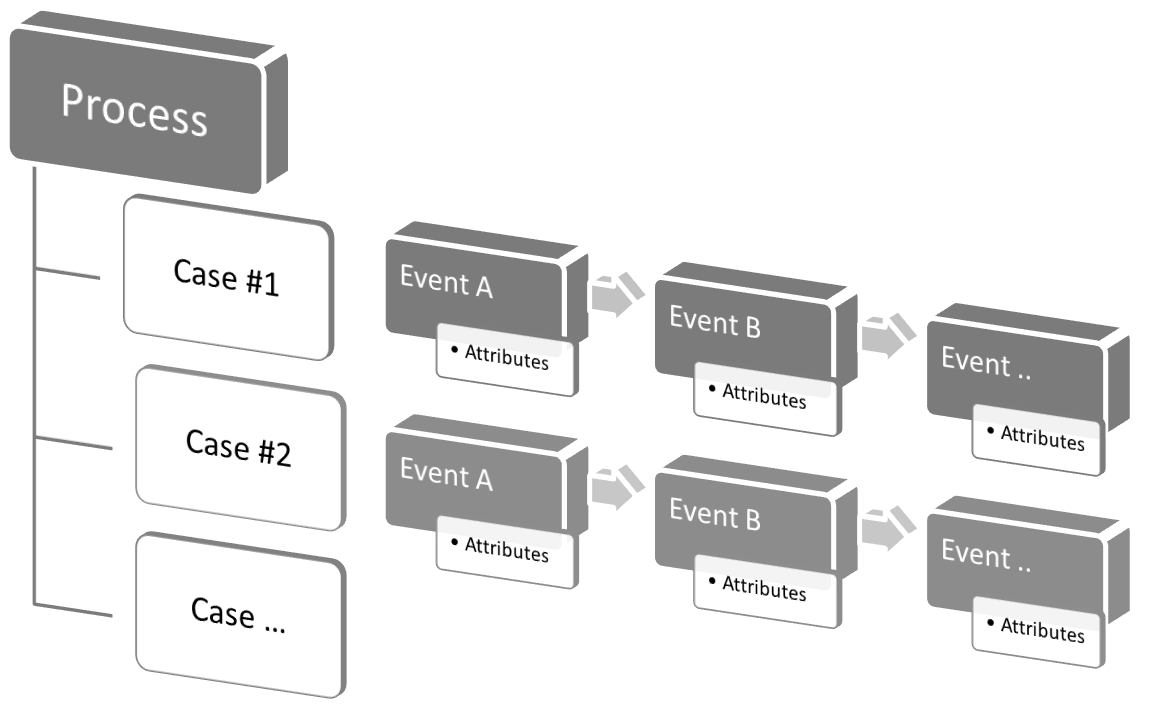
\includegraphics[width=\textwidth]{3_background/event_log_structure}
  \caption{Structure of Event Logs}
  \label{fig:event-log-structure}
\end{figure}

\begin{table}[h]
\centering
\caption{Fragment of event log from Loan Application Process (Variation #1)\cite{loan-app-data}}
\label{table:event-log-loan}
\begin{tabular}{@{}llccc@{}}
\toprule
\multicolumn{5}{c}{\textbf{Event Log}}                                                                  \\ \midrule
                        &                         & \multicolumn{3}{c}{\textbf{Attributes}}             \\ \midrule
                        & \textbf{Event}          & \textbf{Date} & \textbf{Time} & \textbf{Transition} \\ \midrule
\textbf{Case \#1}       & Register Application    & 16.04.2013    & 14:37:27      & Complete            \\ \midrule
                        & Check Credit            & 16.04.2013    & 14:41:19      & Complete            \\ \midrule
                        & Check System            & 16.04.2013    & 14:47:35      & Complete            \\ \midrule
                        & Calculate Capacity      & 16.04.2013    & 14:50:21      & Complete            \\ \midrule
                        & Accept                  & 16.04.2013    & 14:53:22      & Complete            \\ \midrule
                        & Send decision e-mail    & 16.04.2013    & 14:55:11      & Complete            \\ \midrule
\textbf{Case \#2}       & Register Application    & 16.04.2013    & 16:28:19      & Complete            \\ \midrule
                        & Check Credit            & 16.04.2013    & 16:36:22      & Complete            \\ \midrule
                        & Check System            & 16.04.2013    & 16:43:10      & Complete            \\ \midrule
                        & Calculate Capacity      & 16.04.2013    & 16:52:40      & Complete            \\ \midrule
                        & Reject                  & 16.04.2013    & 16:53:53      & Complete            \\ \midrule
                        & Send decision e-mail    & 16.04.2013    & 17:01:32      & Complete            \\ \midrule
\multicolumn{1}{c}{...} & \multicolumn{1}{c}{...} & ...           & ...           & ...                 \\ \bottomrule
\end{tabular}
\end{table}

Event log structure and related notions are formalized in \cite{van2011process} as following:

\theoremstyle{definition}
\begin{definition}{}
(Event and Event Attributes) Let \textit{E} be the universe of events which include all possible event identifiers. In this universe any event \textit{e} $\in$ \textit{E}. Events are enhanced with contextual information, namely attributes. For any event \textit{e} $\in$ \textit{E} and attribute \textit{A}, $\#_\textit{A}(\textit{e})$ is the value of the attribute \textit{A} for event \textit{e}. Possible attributes for events include timestamps, people and resource assignments, transaction types and other contextual data.
\end{definition}

\theoremstyle{definition}
\begin{definition}{}
(Case and Case Attributes) Let \textit{C} be the universe of cases which include all possible case identifiers. In this universe any case \textit{c} $\in$ \textit{C}. Like events, cases are also enhanced with contextual information, namely attributes. For any case \textit{c} $\in$ \textit{C} and attribute \textit{A}, $\#_\textit{A}(\textit{c})$ is the value of the attribute \textit{A} for case \textit{c}. Each case has at least one attribute which is trace.
\end{definition}

\theoremstyle{definition}
\begin{definition}{}
(Trace) Trace is a sequence of event \textit{t} $\in$ $\textit{E}^*$ such that each event is restricted to occur only once.
\end{definition}

\theoremstyle{definition}
\begin{definition}{}
(Event Log) Event log is set of cases \textit{L} $\subseteq$ \textit{C} such that each event occurs at most one in the event log.
\end{definition}

In this study, event logs from different organizations are exploited, thus organization related attributes are used for cases. Within these event logs, traces of cases for each organizational is used to discover underlying process models. In addition, timestamps and resource related attributes of events are used to collect performance related data for further analysis.

\section{Process Modeling}
\label{sec:process-modeling}
Process modeling is the foundation of process management applications and main tools of people in this profession. Although process modeling can be defined with informal process workflows to document procedures, there are a number of formalized notations which are more suitable to cross-applicability and mathematical analysis. In the control-flow view of process modeling, a process model is aimed to give decisions on which activities to take place with their orders. In this study, control-flow of process models are used to find mismatch patterns between different organizations that execute the same activities. Considering the scope of this  thesis, only Petri nets, Workflow Nets and Business Process Modeling Notation(BPMN) will be presented since they are related. 

\subsection{Petri Nets}
\label{sec:petri-nets}
Petri net is a mathematical modeling language that is aimed to describe concurrent systems. Graphical notation of Petri nets seems intuitive and simple; however, it is powerful in terms of being executable and applicability of analysis techniques \cite{vanderAalst:2011:MBP:2000715}. Petri nets are directed bipartite graphs where nodes \textit{represent} transitions and \textit{places} represent conditions. Structure represented by Petri nets is static and the state of the net is described by placing \textit{tokens}, namely the process of \textit{marking}. Formalization of Petri nets are explained in \cite{reisig1998lectures} as following:

\theoremstyle{definition}
\begin{definition}{}
(Petri Nets) A \textit{Petri net} is a triplet $N = (P, T, F)$ where $P$ is finite set of \textit{places}, $T$ is finite set of \textit{transitions} and $F$ is set of \textit{flow relations} where:
\begin{enumerate}
  \item (Separation) $P \cap T = \varnothing$
  \item (Flow relation) $F \subseteq (P \times T) \cup (T \times P)$
\end{enumerate}
\end{definition}


\subsection{Workflow Nets}
\label{sec:workflow-nets}
Process models in the real life have additional properties to be executable and they are defined in the Workflow net formalization, which is simply a subset of Petri nets. These additional properties can be formalized as following \cite{van2013discovering}:
\theoremstyle{definition}
\begin{definition}{}
(Workflow Nets) Let $N = (P, T, F)$ be a Petri net and $t$ is a new identifier not in $P \cup T$. $N$ is a workflow net (WF-net) if and only if:
\begin{enumerate}
  \item (Start Node) $P$ contains a \textit{source place i} where no token can be fired to.
  \item (End Node) $P$ contains a \textit{sink place o} where no token can be fired from.
  \item (Connectedness) $\bar{N} = (P, T \cup \{t\}, F \cup \{(o,t),(t, i)\})$ is strongly connected, in other words there is a directed path between any pair of nodes in $\bar{N}$.
\end{enumerate}
\end{definition}

In simple terms, a Workflow net is a Petri net with a source place to start the process starts and a sink place to end; furthermore, all nodes are on a path from source place to sink place \cite{van1998application}.  In order to illustrate this formalization, the Workflow net for the event log mentioned in Section~\ref{sec:event-log} is presented in Figure~\ref{fig:loan-petri-net}. In the figure, places are indicated by circles, transitions are indicated by rectangles, and flow relations are represented by arcs. 
\begin{figure}
  \centering
  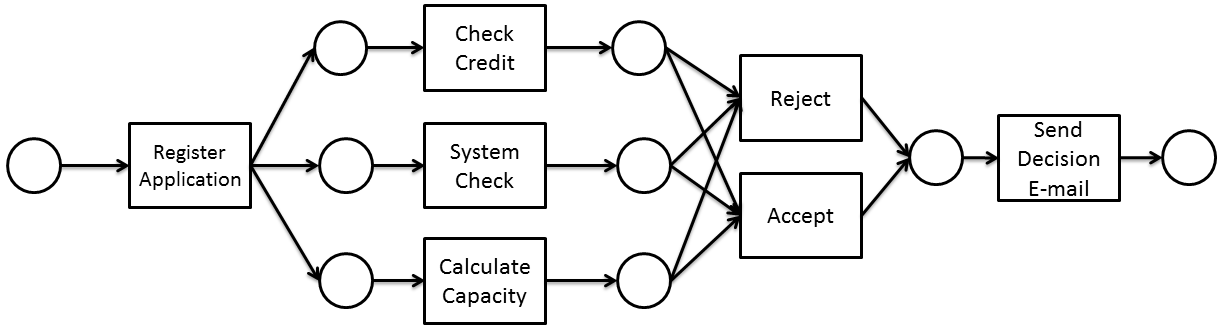
\includegraphics[width=\textwidth]{3_background/loan-petri-net}
  \caption{Workflow net of Loan Application Process (Variation #1)}
  \label{fig:loan-petri-net}
\end{figure}

Workflow nets are representative to real life processes; however, they can result with processes including deadlocks, live-locks and never-reached activities. In order to avoid process models from these problems, soundness definition is suggested in \cite{van1998application} and it is simplified as following with the context of this thesis:
\theoremstyle{definition}
\begin{definition}{}
(Soundness) Let $N$ be a Workflow net and it is sound if and only if:
\begin{enumerate}
  \item  (Safeness) Places cannot hold more than one tokens at the same time.
  \item  (Proper completion) Any marking of net can reach to sink place.
  \item  (Absence of dead tasks) Net does not contain any dead transitions.  
\end{enumerate}
\end{definition}

In this thesis, Workflow nets are used to discover and present underlying process models of different organizations. Considering the applicability of well-known process mining algorithms on Workflow nets and implementations in ProM Framework \cite{verbeek2010prom}, Workflow nets are used as the notation for discovery and analysis.

\subsection{Business Process Modeling Notation (BPMN)}
\label{sec:bpmn} 
Business Process Modeling Notation (BPMN) is one of the most popular and widely used modeling language implemented by many vendors. In addition to its popularity, this notation is standardized by the Object Management Group (OMG) since 2004. In this notation, atomic activities are named as \textit{tasks} and routing decision logic is implemented by \textit{gateways}. These gateways include split and join gateways with AND, OR and XOR logic operations. In addition, deferred choice pattern is implemented by \textit{event-based XOR gateway} in BPMN to handle race conditions between tasks that are running parallel \cite{van2003workflow}. Since the primary goal of BPMN is to provide a standardized notation that is easy to understand by business stakeholders, in this study resulting nets are converted to BPMN diagrams for visual analysis by the plugin implemented in ProM \cite{kalenkovaprocess}. BPMN diagram of the Workflow net from Figure~\ref{fig:loan-petri-net} is presented in Figure~\ref{fig:loan-bpmn}. As can be seen from the diagram, gateways help to understand the relations and dependencies of the tasks.

\begin{figure}
  \centering
  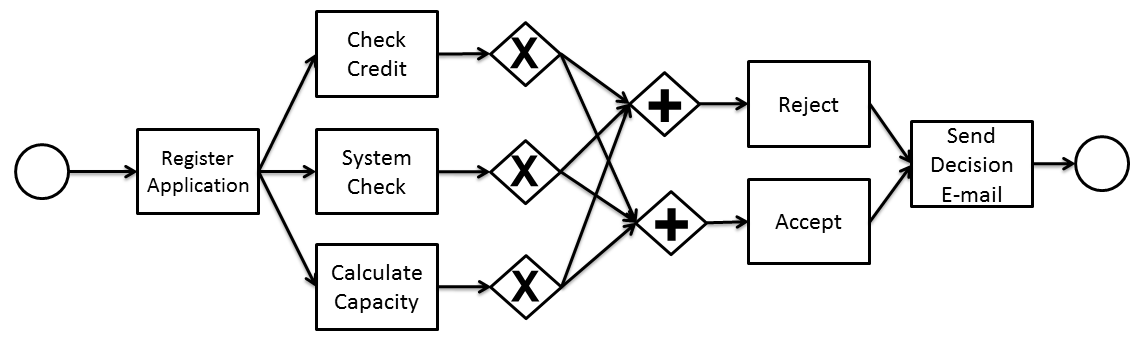
\includegraphics[width=\textwidth]{3_background/loan-bpmn}
  \caption{Process Model of Loan Application Process  (Variation #1) using BPMN}
  \label{fig:loan-bpmn}
\end{figure}


\section{Process Discovery}
\label{sec:process-discovery}
In process mining field, one of the most challenging task is to construct a process model based on the behavior in the event logs, namely process discovery. Many process discovery algorithms are proposed to address different challenges in process discovery and using different notations. However, in this thesis focus of the study is learning from the cross-organizational process mining rather than address all process discovery challenges. With this reasoning, Inductive Process Mining \cite{leemans2013discovering} is selected as appropriate since it is simple, highly applicable and configurable. In the literature, its derivatives which handles infrequent behaviors \cite{leemans2014discoveringinfrequent}; incomplete logs \cite{leemans2014discoveringincomplete}; and model optimization \cite{weidlich2012profiles} are also available.  

\textit{Inductive Miner (IM)}, which is proposed as an extensible framework in \cite{leemans2013discovering}, aims to discover block-structured process models that are sound and fitting to the behavior represented in event log. In addition, this approach focuses on creating rediscoverable models that is a key attribute in this study. Formalization of the key points in the study \cite{leemans2013discovering} are as following:

\theoremstyle{definition}
\begin{definition}{}
(Block-structured Workflow Nets) Block-structured WF-nets are subset of WF-nets where the workflow can be divided recursively into  parts with single entry and exit points.  
\end{definition}

\theoremstyle{definition}
\begin{definition}{}
(Rediscoverability) Let a process is expressible by a model $M$ which is unknown priori. Given a log $L$ of $M$, $L$ is a subset of language used to describe model $M$. $M$ is isomorphic-rediscoverable from $L$ by mining algorithm $B$ if and only if $M \in B(L)$.
\end{definition}
 
Framework developed in the study \cite{leemans2013discovering} uses a divide-and-conquer approach to discover subprocesses of sublogs obtained by splitting the event log. Main steps of the algorithm are listed as following:
\begin{enumerate}
  \item Activity Sets: Split the \textit{activities} in log to disjoint sets.
  \item Sublogs: Split the \textit{log} by using \textit{activity sets}.
  \item Recursive Mining: Mine sublogs with these steps until a sublog contains only single activity.
\end{enumerate}

In the study \cite{leemans2013discovering}, an algorithm based on this framework is presented that guarantees returning a sound and fitting process model in finite time. Therefore, this framework is selected as appropriate and its extension that can handle infrequent behavior which is used within this study to address challenges of different event logs. Frequent behavior is caused by the traces in the logs that might follow many different paths. In real life, these different paths are used infrequently; however, their effect in discovery is still significant. \textit{Inductive Miner Infrequent (IMi)} is proposed in \cite{leemans2014discoveringinfrequent} as an extension to \textit{Inductive Miner} to handle noise in the event logs. By filtering the infrequent behavior, it is aimed that \textit{IMi} succeeds with improved models discovered. After each recursive step of \texit{IM}, filtering is applied if the discovered model is a flower model which represents infrequent behavior. Basic idea behind filtering is considering the trace and event frequency with a user-defined threshold between 0 to 1. Using this threshold, both log splittings and mining operations are done on a cleaner subset of logs. When the discovered models compared to \textit{IM}, \textit{IMi} results with lower fitness, higher precision and equal generalization.
In this thesis study, infrequent behavior capable implementation is used for experimenting the cross-organizational mining of process models with their implementation of ProM framework \cite{verbeek2010prom}.

\section{Process Performance Analysis}
\label{sec:process-performance-analysis}
\todo{WRITE}
% burayı 2.3.2'den performance ile enhance et

\section{Machine Learning and Clustering}
\label{sec:unsupervised-learning}
Machine learning is a study area of computer science which have roots in pattern recognition and computational learning theory of artificial intelligence. Machine learning approaches works on construction and learning from data to make further predictions. There are various approaches proposed in this area and clustering approach will be presented in this section. Cluster analysis is based on assigning the set of observations into subsets (\textit{clusters}) so that observations within the same cluster are similar whereas the observations from different clusters are dissimilar, where the similarity criteria is predefined. Clustering is a method in unsupervised learning, where the main problem is learning a hidden structure in unlabeled data. Since the provided data is unlabeled there is no error or reward assignment to the potential solutions provided these approaches; however, quality metrics on clusters are used to evaluate results. With these characteristics, clustering is a common technique in exploratory data mining and statistical data analysis and it is used in many fields like image analysis, information retrieval and bioinformatics.

In cluster analysis, various algorithms are proposed with different notions on defining clusters and how to efficiently find them. Popular approaches are based on the idea of decreasing the distance among the members of same cluster, space density of data space, intervals or particular statistical distributions. Within this thesis study, centroid-based clustering is used in which the clusters are defined by a central vector, which may not a member of data set. When number of clusters are fixed to \textit{k}, the approach is named as \textit{k-means clustering} and the problem is finding k cluster centers and assigning data members to nearest cluster center while minimizing the squared distances of data members to the assigned cluster centers. Although seems easy, this optimization problem is NP-hard and most of the implementations include approximate solutions. A well-known algorithm in k-means clustering is Lloyd's algorithm and it is referred as \textit{k-means algorithm} and its variation based on random initialization \textit{k-means++} are formalized in the study of Arthur and Vassilvitskii \cite{arthur2007}:
 
\theoremstyle{definition}
\begin{definition}{k-means Algorithm}
\begin{enumerate}
  \item Arbitrarily choose initial $k$ centers: $C={c_1,c_2,...c_k}$
  \item For each $i \in {1,...k}$, set the cluster $C_i$ to be the set of points that are closer to $c_i$ than they are to $c_j$ for all $i\neqj$.
  \item For each $i \in {1,...k}$, set $c_i$ to be the center of mass of all points in $C_i$. $c_i=\frac{1}{|C_i|} \sum_{\substack{x\in C_i}} x$
  \item Repeat Step 2 and 3 until $C$ no longer changes.
\end{enumerate}
\end{definition}

\theoremstyle{definition}
\begin{definition}{k-means++ Algorithm}
\begin{enumerate}
  \item Take one center $c_1$, chosen uniformly from data points $X$.
  \item Take a new center $c_i$, chosen from data points $X$ with probability $\frac{D(x)^2}{\sum_{\substack{x\in X}} D(x)^2}$ where let $D(x)$ is the shortest distance from a data point to the closest cluster center.
  \item Repeat Step 2 until $k$ cluster centers are selected.
  \item Proceed with the 2-4 steps of k-means Algorithm.
\end{enumerate}
\end{definition}


In this thesis study, clustering of performance analysis results is undertaken and since the number of data instances low an approach focused on initialization is selected. Implementation of \textit{k-means++} in WEKA (Waikato Environment for Knowledge
Analysis) \cite{hall2009} is used as Java API to call from ProM Framework \cite{verbeek2010prom}. 

\section{Mismatch Patterns in Process Models}
\label{sec:mismatch-patterns-in-process-models}

In cross-organizational process mining environment, there is a need to align processes of different organizations and in this scope both the organizations and their processes are similar but have significant differences. In order to align these processes and organizations, there is a need for spotting differences between process models. In the study of Dijkman \cite{dijkman2007mismatch}, a collection of patterns to describe frequent mismatches between the similar process models are presented. Mismatch patterns are grouped into three as authorization, activity and control flow mismatch patterns. Authorization mismatch patterns are based on assignment of the same tasks to different roles in different processes and left outside the scope of this thesis. Activity mismatch patterns are based on representing the tasks of a process by a different collection of activities in a different process, or not representing at all. Within the scope of this study, the related mismatch patterns are defined in study \cite{dijkman2007mismatch} as following:

\todo{draw diagrams}
\begin{description}
  \item[Skipped Activity] An activity exists in one process but no equivalent activity is found in the other process as illustrated in Figure~.
  \item[Interchanged Activity] An activity exists in one process but as an equivalent another activity is found in the other process to achieve the same task as illustrated in Figure~.
  \item[Refined Activity] An activity exists in one process but as an equivalent a collection of activities are existing in the other process to achieve the same task. An illustration is provided in Figure~. 
\end{description}
 
Control flow mismatch patterns are based on using different control-flow relations and dependencies for the same activities in different processes. Within the scope of this study, the following control flow mismatch patterns are defined in study \cite{dijkman2007mismatch}:

\begin{description}
  \item[Activities at Different Moments in Processes] Set of activities are undertaken with different orders in different processes as shown in Figure~.
  \item[Different Conditions for Occurrence] Set of dependencies are same for two processes; however, occurrence condition is different. An example is provided in Figure~.
  \item[Different Dependencies] Set of activities have differ in their dependency sets. An example of this pattern is shown in Figure~.
  \item[Additional Dependencies] This pattern is a special case of different dependencies where one set of activities includes the other and results with additional dependencies as illustrated in Figure~.
\end{description}


As mentioned in the study \cite{dijkman2007mismatch}, their approach does not create a comprehensive list to resolve all mismatches but the most common ones spotted during case studies. In addition, there are no algorithms provided to spot these mismatches in \cite{dijkman2007mismatch} or consequent studies, and thus implementation of spotting mismatch patterns are kept within the scope of this thesis study. 
\chapter{METHODOLOGY}
\label{chp:methodology}

In this chapter, methodology proposed in this thesis study is presented. Firstly, approach overview is described from a high-level perspective. Then, each stage in the methodology is presented together with their importance in the study, mathematical representations and definitions; and black-box diagrams. In the last section of this chapter, implementation details of this methodology in ProM framework is explained in detail with a software architecture overview.

\section{Approach Overview}
\label{sec:approach-overview}
Approach proposed in this study consists of four main stages and general information about these stages can be summarized as following:
\begin{description}
	\item[Process Model Mining:] Process models are extracted from event logs for each organization with a user specified noise threshold.
	\item[Performance Indicator Analysis:] Event logs are replayed on process models and performance indicators are calculated for each organization. Using these indicators, organizations are clustered based on how well they are operating.
	\item[Mismatch Pattern Analysis:] Differences between process models of organization are extracted with a well-established mismatch patterns.
	\item[Recommendation Generation:] Using the performance indicator clusterings and differences between process models, a set of recommendation for each organization is generated.
\end{description}

Flow of these stages with the important input and outputs can be visualized in Figure~\ref{fig:approach-overview}. In the following sections, each stage will be explained in detail with their mathematical backgrounds.
\begin{figure}
  \centering
  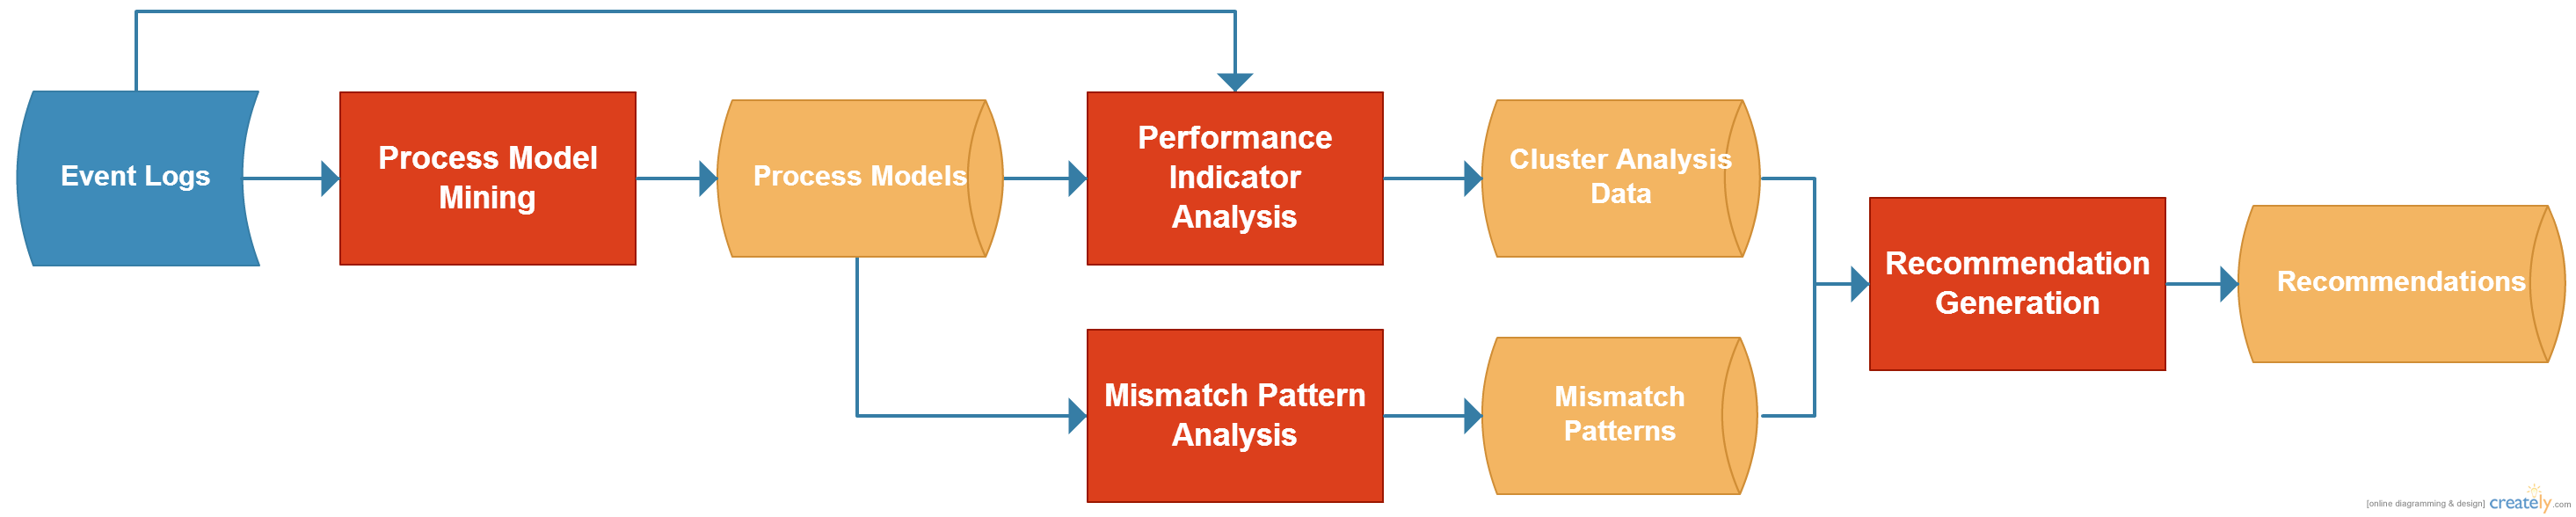
\includegraphics[width=\textwidth]{4_methodology/approach-overview}
  \caption{Overview of Methodology}
  \label{fig:approach-overview}
\end{figure}

\section{Process Model Mining}
\label{sec:process-model-mining}
Process model mining stage in the proposed approach has the aim of creating reproducible and generalized process models from event logs. In order to achieve this aim, implementation of \textit{Inductive Miner Infrequent (IMi)}, which is proposed in \cite{leemans2014discoveringinfrequent} as an extension to \textit{Inductive Miner} to handle noise in the event logs, is used in this study. 

The selected implementation has the ability of pruning data to handle noise in the event logs. Like the other data mining approaches, event logs include data related to the infrequent behaviors occurred in real life. Although these infrequent behaviors might be caused by important structural or case related issues that should be analyzed; they make the process of mining and results more complex. In the scope of this study, without cleaning the data, most of the process model mining approaches result with \textit{spaghetti-like models} \cite{van2011process} which are difficult to further analyze. Since this thesis focuses on learning from the cross-organizational process mining rather than creating the best-fitting process models, data cleaning and noise handling is a necessary step. Therefore preprocessing steps are undertaken with a compatible approach of \textit{Inductive Miner Infrequent (IMi)}, where data is cleaned in every inductive step.

Considering the scope of this study, instead of computational details of \textit{Inductive Miner Infrequent (IMi)} black-box representation is used to explain its usage in the methodology. In order to provide a filtering threshold, a user-provided value between 0 to 1 is added as input to method in addition to event logs. As a result, workflow net is produced which is a sound and properly completed Petri net without deadlocks. Black-box of this stage is illustrated in Figure~\ref{fig:process-model-mining-blackbox} and this stage is called for every organization's event logs to create their own process models in Workflow net formalization.

\begin{figure}
  \centering
  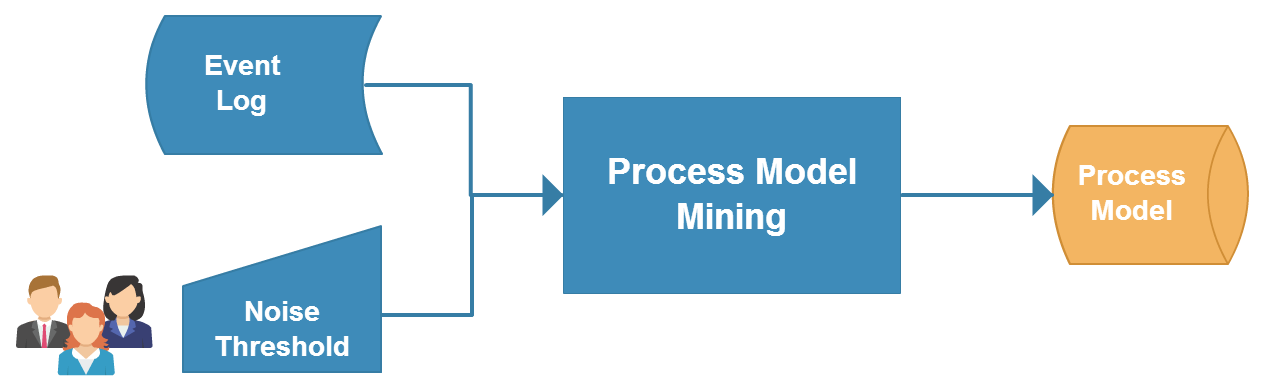
\includegraphics[width=\textwidth]{4_methodology/process-model-mining-blackbox}
  \caption{Process Model Mining Stage as Black-box }
  \label{fig:process-model-mining-blackbox}
\end{figure}


\section{Performance Indicator Analysis}
\label{sec:performance-indicator-analysis}
Performance indicator analysis stage focuses on calculating and analyzing the performance values using the event logs and mined process models. This stage consists of mainly two concepts as 
\begin{inparaenum}[\itshape a\upshape)]
\item alignment and calculation of performance indicators; and
\item clustering of organizations based on their performance values.
\end{inparaenum}
In order to evaluate the performance of an organization based on their process models and past activities; there are a number of indicators in time dimension, cost dimension and utilization \cite{van2011process}. However, in this study, process related performance values are considered since differences in the process models are studied in the next stages. With this reasoning, the following performance indicators are calculated and analyzed in this stage of methodology:
\begin{description}
  \item[Average Time Between Activities] For each activity in the process model, average time to reach other activity is calculated. This is a simple but powerful performance metric for organizations since it can yield the average time to complete one task based on a starting point. From the performance perspective, organizations want to minimize average time between activities to increase their throughput \cite{van2012replaying}. This notion can be defined as following:
	\theoremstyle{definition}
	\begin{definition}{}
	Average time between activity $A$ and $B$ in organization $i$ is 
	$AvgTime_{A\rightarrow B}^{i} = \sum_{Case\ c \in Event Log_{i}} TimeBetween_{c}(A,B) / Occurences_{Event\ Log_{i}}(A,B)$ where
		\begin{enumerate}
			\item $TimeBetween_{c}(A, B) = EndTime_{c}(B) - StartTime_{c}(A)$
			\item $StartTime_{c}(A)$ is start time of activity $A$ in case $c$,
			\item $EndTime_{c}(B)$ is end time of activity $B$ in case $c$,
			\item $Occurences_{Event Log_{i}}(A, B)$ is number of occurrences of  activity $A$ followed by $B$ in  $Event\ Log_{i}$.
		\end{enumerate}
	\end{definition}

	\item[Standard Deviation of Time Between Activities] Time between activities in real life is not stable and they deviate due to various reasons such as people responsible of tasks, size and the content of tasks or seasonality \cite{van2011process}. On the other hand, organizations want to be confident about their processes and therefore they want to minimize the deviation in the time between activities. Minimized deviation in time helps organizations to plan, act and re-organize the activities in the processes with high accuracy \cite{van2012replaying}. With the same approach above, the following formulation can be defined:
	\theoremstyle{definition}
	\begin{definition}{}
	Standard deviation time between activity $A$ and $B$ in organization $i$ is 

	$StdDevTime_{A\rightarrow B}^{i} = \sqrt{\frac{\sum_{Case\ c \in Event Log_{i}} [TimeBetween_{c}(A, B) - AvgTime_{A\rightarrow B}^{i}]^{2}}{Occurences_{Event\ Log_{i}}(A,B)} }$ 
	\end{definition}
\end{description}

In addition to average and standard deviation, minimum and maximum times between activities can also be analyzed. However, these performance values are mostly result of rare cases in the event logs and these rare occurrences have the probability of being eliminated as noise in process mining stage. Therefore, the minimum and maximum values have the risk of not representing the actual performances. Thus, only average and standard deviation of the time between activities are selected in the study. 

\subsection{Replay and Performance Indicator Calculation}
\label{subsec:replay-and-performance-summary}
Replay of event logs on process models is based on the idea of \textit{alignment} which is formalized in \cite{van2012replaying} and the basic assumption in this concept is that process models and event logs have the same activity labels. Alignment is based on \textit{moves in the model and log} and in order to have a successful replay where optimal alignment should be achieved. As proposed in \cite{adriansyah2011conformance} \cite{adriansyah2011towards}, $A^{*}$ algorithm which is a path-finding algorithm based on graphs is used to find optimal alignment of event logs on the process models.

In order to appropriately apply $A^{*}$ algorithm, there are number of manual and computational steps that should be undertaken. The following prerequisite steps are implemented in \cite{adriansyah2011towards} to apply $A^{*}$ algorithm:
 \begin{description}
	\item[Set Label Patterns between Process Model and Event Log:] In the event logs, there are various different transitions of the same activity which are generally not represented in process models. For instance, there can be \textit{"Activity A, Start"} and \textit{"Activity A, End"} in the event log; however they are reflected as \textit{"Activity A"} in the process model. Therefore, a list of all transitions and events are asked to the user to match to the ones in the process model in terms of patterns or regular expressions.
	\item[Create Initial and Final Markings:] In case of there is no definite starting or ending point in the process model, user input is necessary to define these activities.
	\item[Set Cost Values:] Since $A^{*}$ algorithm is based on alignments which are basically moves along process models and event logs, the following cost values for each move is necessary to be set:
	\begin{inparaenum}[\itshape a\upshape)]
		\item move on process model, 
		\item move on event log; and
		\item synchronous move.
	\end{inparaenum}
\end{description}
In order to use replay as an intermediate stage in this thesis, some of the mentioned steps are automatized with the help of the assumptions in the prior and post stages of methodology. With this reasoning, initial and final markings are created with the first and last activities in the process models. In addition, since there is no explicit priority of process model over event log or vice versa, cost values are set to 1 for both \textit{move on process model} and \textit{move on event log}. Since there is no penalty for \textit{synchronous moves}, their cost value is set to 0. However, since each event log has different set of transition labels, manual user input is still necessary to map label patterns between process model and event log. With the generated and user-specified inputs, replay and performance indicator calculation in the methodology can be visualized in Figure~\ref{fig:replay-and-performance-indicator-calculation}. For each organization, the steps in the diagram are followed with the corresponding event logs and process models; and the resulting process summaries are used for further analysis.

\begin{figure}
  \centering
  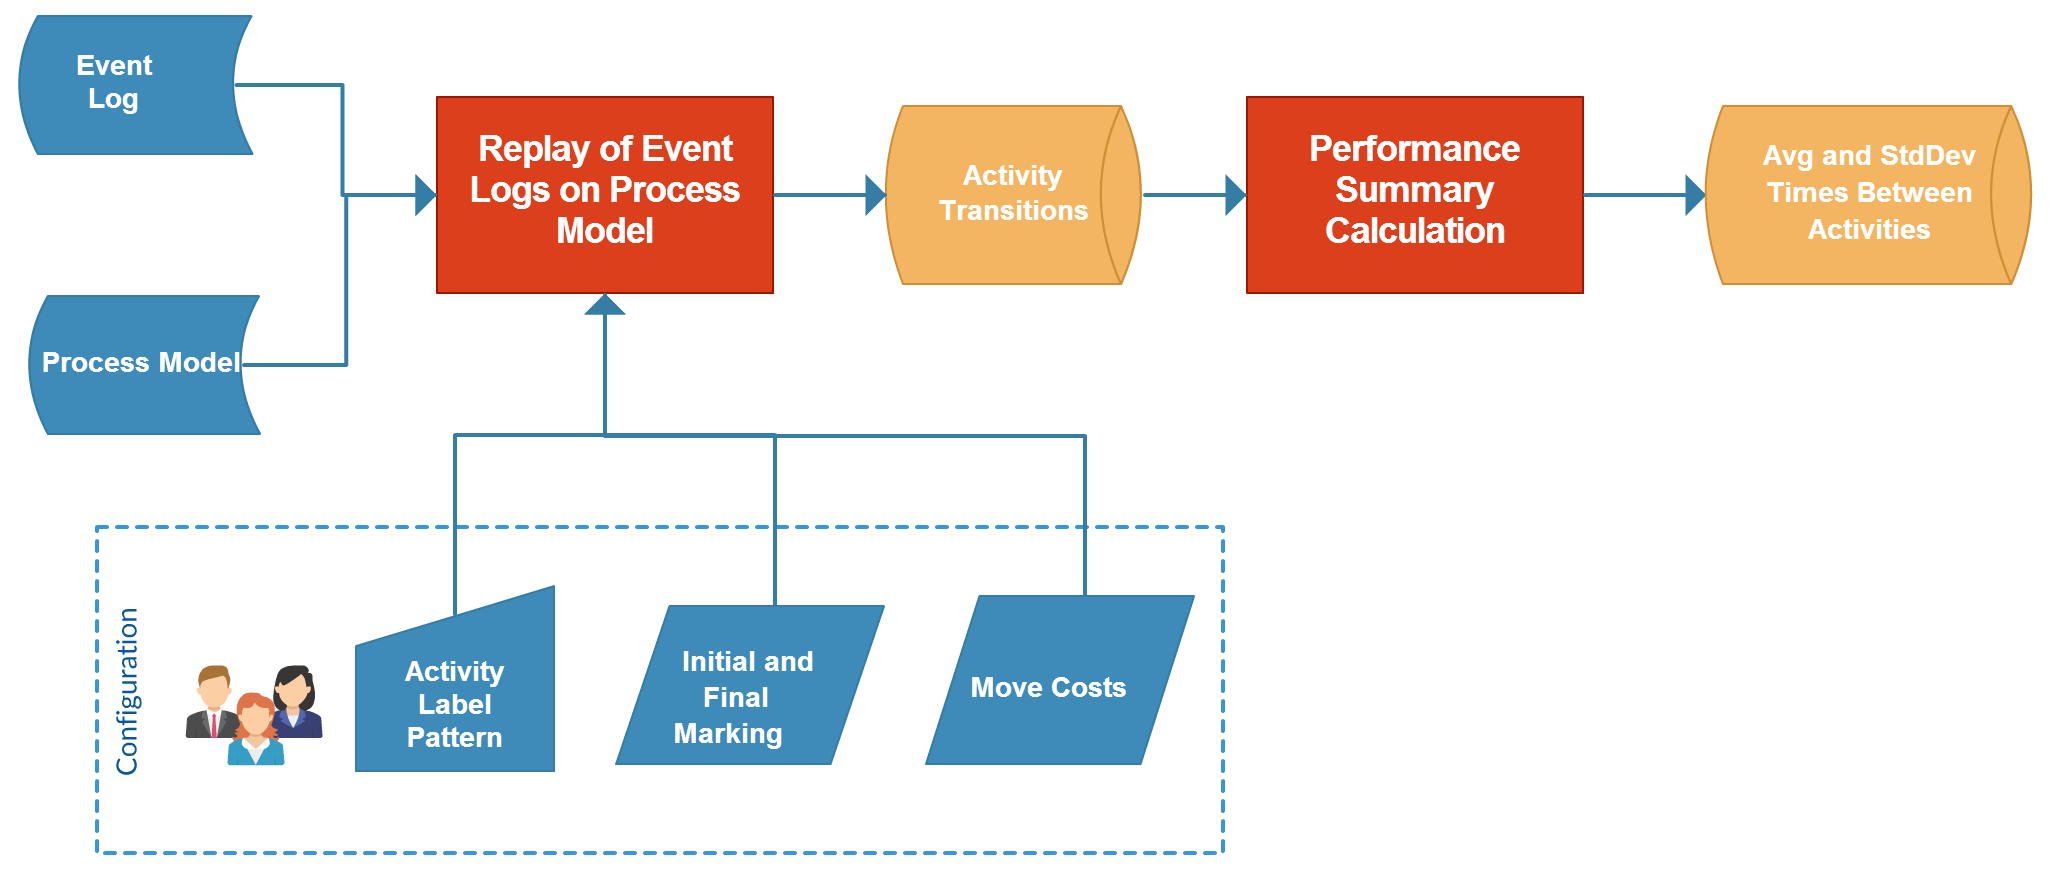
\includegraphics[width=\textwidth]{4_methodology/replay-and-performance-indicator-calculation}
  \caption{Replay and Performance Indicator Calculation Stage as Black-box}
  \label{fig:replay-and-performance-indicator-calculation}
\end{figure}

Performance summary calculation step at the end of this stage is used to create a summary of data consists of average and standard deviation of time between activities. Resulting data can be defined as following:
	\theoremstyle{definition}
	\begin{definition}{} Performance Summary data for any organization $i$ is 

	$PerfSum_{i}= \{AvgTimeSum_{i}\ \cup\ StdDevTimeSum_{i}\}$ where
		\begin{enumerate}
			\item $AvgTimeSum_{i} = \{ AvgTime_{A \rightarrow B}^{i} | A , B  \in Event\ Log_{i}\}$
			\item $StdDevTimeSum_{i} = \{ StdDevTime_{ A\rightarrow B}^{i} | A, B  \in Event\ Log_{i}\}$
		\end{enumerate}
	\end{definition}

\subsection{Performance Indicator Clustering}
\label{subsec:performance-indicator-clustering}

Clustering is based on the idea of collecting the set of observations into clusters so that observations within the same cluster are similar whereas the observations from different clusters are dissimilar. Being a unsupervised learning method, it aims to find hidden structures in unlabeled data. In this thesis study, clustering is used to cluster organizations based on their performance indicator data. In other words, organizations will be set into groups based on how much time in average and with variation takes to complete an activity given a starting point.

Within clustering analysis, various algorithms are proposed to find clusters based on the idea of decreasing in-cluster distances, increasing space density or fitting to particular statistical distributions. However, in this study, a generic approach based on centroid-based clustering is exploited. For the fixed number of \textit{k} clusters, the approach is well-known as \textit{k-means clustering}. Considering the popularity of this approach and its extensions, random initialization based \textit{k-means++} approach from the study of Arthur and Vassilvitskii \cite{arthur2007} is used to cluster organizations. 

Clustering methods can be evaluated by the internal and external methods. Internal methods are based on the data that is clustered itself whereas external methods use the additional information such as labels or benchmarks. Although there are various well-established metrics in external methods such as Rand Measure, F-measure, Jaccard index or Confusion Matrices; in this thesis study there is no pre-labeled organizations based on their performance indicators. Therefore, internal evaluation methods are used to assess the quality of clusters. Considering the fact that actual data to cluster is \textit{time interval} and centroid-based clustering is applied in this study, a metric based on decreasing the in-cluster distances is selected. With this consideration, Sum of Squared Error (SSE) is calculated with the following definition. When the clustering results are compared, it is reasonable to choose the one with the least SSE; however, it is a fact that as \textit{k} converges to the number of original sample size SSE value decreases. Therefore, SSE values and number of clusters are plotted and presented to the end user of the methodology to select optimal number of clusters.

\theoremstyle{definition}
\begin{definition}
Sum of Squared Error (SSE) is

$SSE = \sum_{i=1}^{k} \sum_{x \in c_{i}} EuclideanDistance(mean_{i}, x)^{2}$ where
\begin{enumerate}
  \item $x$ is a data point in cluster $c_{i}$.
  \item $mean_{i}$ is the mean vector of the cluster $c_{i}$.
\end{enumerate}
\end{definition}

For each organization, \textit{Performance Summary} data is used as the data source in clustering. It is aimed that the organizations with the similar average or standard deviation time between tasks will be assigned to same sets to further reveal the dissimilarities that the other clusters can learn from. Since not every activity exists in every organization, performance summary data is cleaned and merged to include only all shared activities. This cleaning step removes the non-existing activity related performance indicators from all the organizations so that clustering is applied on the data with no process model related information. Since number of clusters are not known priori, k-means clustering is applied starting \textit{k} from 1 to the number of organizations. For each clustering with different number of clusters, SSE values are plotted and user is made to select the appropriate cluster size. For the selected cluster size, clustering related information is used to generate recommendations in the further steps. This stage of methodology can be visualized as an input-output system in Figure~\ref{fig:performance-indicator-clustering-blackbox}. Resulting cluster analysis data is formulated as following:

\theoremstyle{definition}
\begin{definition}
Cluster Analysis Data is a tuple $(k, Assignments, Cluster\ Centroids)$ where
\begin{enumerate}
	\item $k$ is the number of clusters,
	\item $Assignments$ is a set of tuple $(Organization_{i}, Cluster_{j})$ where $i$ is identifier for organization and $j \leq k$ is identifier for cluster,
	\item $Cluster\ Centroids$ is a set of tuple $(Cluster_{j}, Type, A_{start}, A_{end}, Value)$ where
		\begin{enumerate}
			\item $Type$ is performance indicator type which is $Average$ or $StandardDev$,
			\item $A_{start}$ and $A_{end}$ are starting and ending points of performance indicator,
			\item $Value$ is the actual value of performance indicator,
			\item $Cluster\ Centroids_{j}$ is a function that returns set of $Centroid$ which are tuples of $(Type, A_{start}, A_{end}, Value)$ for $Cluster_{j}$.
		\end{enumerate}	
\end{enumerate}
\end{definition}
 
\begin{figure}
  \centering
  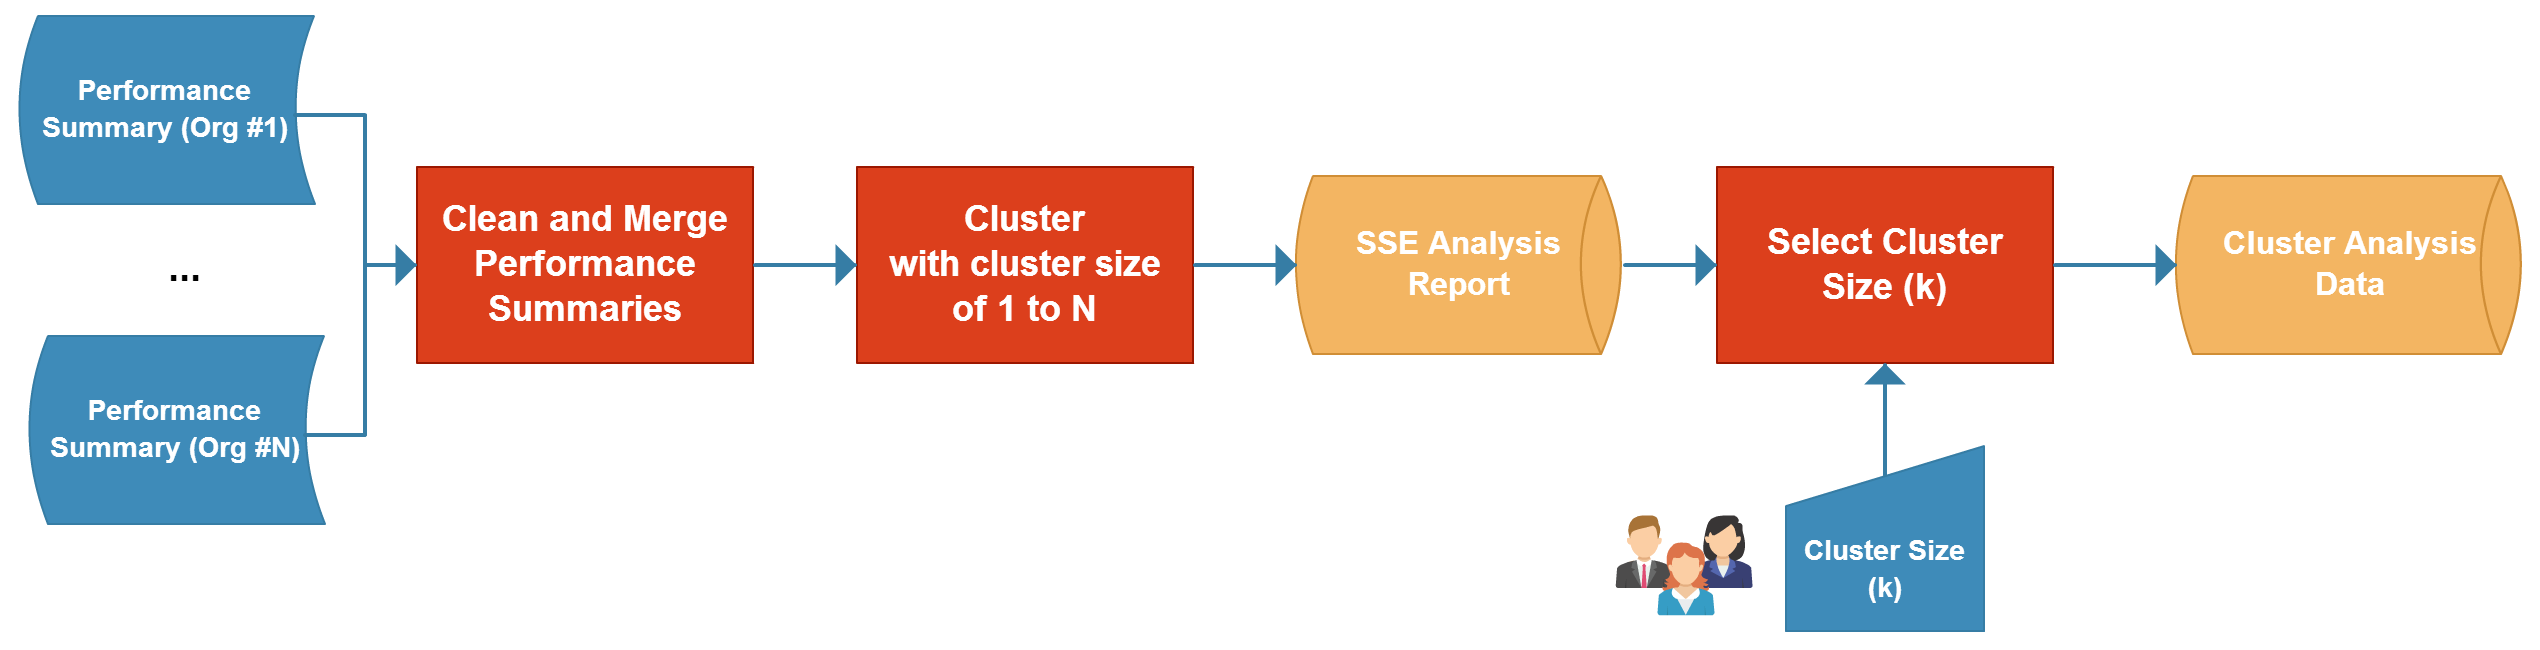
\includegraphics[width=\textwidth]{4_methodology/performance-indicator-clustering-blackbox}
  \caption{Performance Indicator Clustering Stage as Black-box }
  \label{fig:performance-indicator-clustering-blackbox}
\end{figure}
 
\section{Mismatch Pattern Analysis}
\label{sec:mismatch-pattern-analysis}
In order to learn from other organizations, it is necessary to spot the differences between process models of different organizations. In this phase of methodology, differences between process models will be revealed by the mismatch patterns which are defined by Dijkman \cite{dijkman2007mismatch}. In the process mining stage, process models are mined to create Workflow nets; however, mismatch pattern definitions are closer to business environment and it is more suitable spot patterns in BPMN notation. Thus, mined process models are converted to BPMN models and then mismatch pattern analysis is applied. After spotting differences, mismatch patterns for activities and control flows average revealed for the organizations.

Business Process Modeling Notation (BPMN) is one of the widely accepted modeling language in the industry and its a standardized notation by the Object Management Group (OMG) since 2004. Main aim of BPMN is to provide a notation that is easily understood by business stakeholders. In the preceding stages, Petri nets and their subset as Workflow nets are used for mining since they have stronger mathematical background. However, in this stage, BPMN formulation is used since mismatch patterns have roots in real-life business environment \cite{dijkman2007mismatch}. The following definition and conversion are defined in the study \cite{kalenkovaprocess} and they are used in the mismatch pattern analysis. 

\theoremstyle{definition}
\begin{definition}
A BPMN model is a tuple 

$BPMN_{model}=(N, A, G_{XOR}, G_{AND}, e_{start}, E_{end}, SF, \lambda)$ where
\begin{enumerate}
  \item $N$ is a set of flow nodes,
  \item $A \subseteq N$ is a set of activities,
  \item $G_{XOR} \subseteq N$, $G_{AND} \subseteq N$ are sets of exclusive and parallel gateways,
  \item $e_{start} \in N$ is a start event,
  \item $E_{end} \in N$ is a set of end events,
  \item Sets $A, G_{XOR}, G_{AND}, \{e_{start}\}, E_{end}$ form a partition of N,
  \item $SF \subseteq N \times N$ is a set of sequence flows,
  \item $\lambda : N \rightarrow U_{A}$ is a labeling function, where $U_{A}$ is some universe of activity labels,
  \item Start event $e_{start}$ does not have incoming sequence flows and has not more than one outgoing sequence flows,
  \item End events $E_{end}$ do not have outgoing sequence flows.  
\end{enumerate}
\end{definition}

\theoremstyle{definition}
\begin{definition}
Constructing BPMN Model from Petri nets, which are $N = (P, T, F)$ where $P$ is finite set of \textit{places}, $T$ is finite set of \textit{transitions} and $F$ is set of \textit{flow relations} to BPMN models consists of the following steps:
\begin{enumerate}
  \item Initialize BPMN model with a start node $e_{start}$.
  \item Convert all transitions, $T$, in the Petri net by creating an activity in BPMN model for each transition in Petri net.
  \item Convert all places, $P$, from Petri net to BPMN routing constructs by finding the corresponding sequence flows.
\end{enumerate}
\end{definition}

For each organization, mined process models are converted to BPMN models and mismatch patterns analysis is undertaken on them. For each mismatch pattern analysis, the aim is to locate differences between two process models or cluster of process models. In addition, since performance indicators are calculated based on a starting and ending point in the process model, same approach is applied to locate mismatch patterns. In other words, differences of process models are located through a starting activity to an ending activity. This approach also enables to locate the whole set of mismatches between process models when starting and ending points are provided as source and sink activities. Mismatch patterns are formulated and their importance in the methodology are listed as following:
\begin{description}
  \item[Skipped Activity] Skipped activities are the operations that are not undertaken with some of the organizations. In business environment there could be various different reasons for an organization to exclude any activity in their process flows which are followed by other organizations. Therefore, this mismatch pattern should not be utilized solely but taken in to care with the other patterns. In this study, for each organization a list of activities that they do not include are listed as \textit{Skipped Activity} with the following definition. In addition, these differences are checked for the activities with a particular start and end point. 
		\theoremstyle{definition}
		\begin{definition}
		Skipped Activity pattern is a tuple 

		${Skipped\ Activity} = (O, SA, A_{start}, A_{end}) $ where 
		\begin{enumerate}
		  \item $O$ is the identifier for organization,
		  \item BPMN model of organization is $BPMN_{O}$ and $BPMN_{*}$ is the set of all BPMN models in analysis,
		  \item $SA$ is a set of skipped activities and $SA =  BPMN_{*}(A) \setminus BPMN_{O}(A)$,
		  \item $A_{start}$ and $A_{end}$ are starting and ending points to check mismatch patterns and $A_{start}, A_{end} \in BPMN_{O}(A)$.
		\end{enumerate}
		\end{definition}

		\theoremstyle{definition}
		\begin{definition}
		Skipped Activity Analyzer is a function 

		$SkippedActivityAnalyzer(O, A_{start}, A_{end})$ and it returns a set of \textit{Skipped Activity} for the organization $O$ and the activities between $A_{start}$ and $A_{end}$.
		\end{definition}
  \item[Refined Activity] Refined activities exist in one process; however, as equivalent a collection of activities are undertaken in another organization's process to achieve the same task. Since there is no activity ontology information is kept in event logs and process models, there is no direct method to define whether the tasks can be classified as other tasks' refined state. In this study, assuming the labels of activities are correct and explanatory about their enclosures, similarity between labels are utilized for this aim. Using \textit{Levenshtein distance}, which is very popular in information retrieval area and also known as \textit{edit distance}, similarity of activity labels are calculated for each activity in respect to activities of other organizations' process models. This mismatch pattern presents information about the similar but not same activities in different process models which can be used to make organizations learn from each other. With a user-defined threshold for similarity based on the nature of business environment, most similar tasks can be listed for being refined.
		\theoremstyle{definition}
		\begin{definition}
		Refined Activity pattern is a tuple 

		${Refined\ Activity} = (O_{1}, O_{2}, RA, SimilarityMap, A_{start}, A_{end}) $ where 
		\begin{enumerate}
		  \item $O_{1}$ is the first organization where the refined activity is undertaken with the BPMN model of $BPMN_{{O}_{1}}$,
		  \item $O_{2}$ is the second organization where a collection of activities checked for similarity with the BPMN model of $BPMN_{{O}_{2}}$,
		  \item $RA$ is the refined activity and $RA \in BPMN_{{O}_{1}}(A)$ and $RA \notin BPMN_{{O}_{2}}(A)$,
		  \item $SimilarityMap$ is a set of tuples $(SimilarityValue, A)$ where $SimilarityValue$ indicates the similarity between $RA$ and $A \in BPMN_{{O}_{1}}(A)$, 
 		  \item $A_{start}$ and $A_{end}$ are starting and ending points to check mismatch patterns and $A_{start}, A_{end} \in BPMN_{{O}_{1,2}}(A)$. 
		\end{enumerate}
		\end{definition}

		\theoremstyle{definition}
		\begin{definition}
		Refined Activity Analyzer is a function 

		$RefinedActivityAnalyzer(O_{1}, O_{2}, A_{start}, A_{end})$ and it returns a set of \textit{Refined Activity} for the organization $O_{1}$ compared to $O_{2}$ for the activities between $A_{start}$ and $A_{end}$.
		\end{definition}

   \item[Activities at Different Moments in Processes] Activities at different moments means that organizations are undertaking activities at different orders in their process flows. This mismatch pattern indicates that the organizations could achieve the same task when they change the order of activities and this information can be used by others to enhance their process models. Therefore, formulation of this pattern includes an activity; and its previous and next tasks at different organizations.
		\theoremstyle{definition}
		\begin{definition}
		Activities at Different Moments in Processes pattern is a tuple 

		${Different\ Moments} = (O_{1}, O_{2}, A, Prev_{1}, Next_{1},Prev_{2}, Next_{2}, A_{start}, A_{end}) $ where 
		\begin{enumerate}
		  \item $O_{1}$ is the first organization with the BPMN model of $BPMN_{{O}_{1}}$,
		  \item $O_{2}$ is the second organization with the BPMN model of $BPMN_{{O}_{2}}$,
		  \item $A$ is the activity that is undertaken in different order and $A \in BPMN_{{O}_{1,2}}(A)$,
		  \item $Prev_{1}, Next_{1},$ are previous and next tasks of $A$ in $O_{1}$ and  $Prev_{1}, Next_{1} \in  BPMN_{{O}_{1}}(A)$,
  		  \item $Prev_{2}, Next_{2},$ are previous and next tasks of $A$ in $O_{2}$ and  $Prev_{2}, Next_{2} \in  BPMN_{{O}_{2}}(A)$,
  		  \item In order to ensure different moments $Prev_{1} \neq Prev_{2}$ or $Next_{1} \neq Next_{2}$,
 		  \item $A_{start}$ and $A_{end}$ are starting and ending points to check mismatch patterns and $A_{start}, A_{end} \in BPMN_{{O}_{1,2}}(A)$. 
		\end{enumerate}
		\end{definition}

		\theoremstyle{definition}
		\begin{definition}
		Different Moments Analyzer is a function 

		$DifferentMomentsAnalyzer(O_{1}, O_{2}, A_{start}, A_{end})$ and it returns a set of \textit{Different Moments} for the organization $O_{1}$ compared to $O_{2}$ for the activities between $A_{start}$ and $A_{end}$.
		\end{definition}

	\item[Different Conditions for Occurrence] Different conditions for occurrence take place where an activity has the same dependencies in different organizations but with different conditions. For instance, an organization needs to complete all dependency tasks before starting the next one; though another organization checks for the completion of only one of these dependencies. This difference between organizations can lead to loosen or tighten the conditions based on the application of other organizations. Considering the representation of different conditions for occurrence and other control flow mismatch patterns, a generic definition is developed firstly to use and further customize. Different conditions for occurrence pattern definition is developed based on this generic definition as following.
		\theoremstyle{definition}
		\begin{definition}
		Control Flow Mismatch pattern is a tuple 

		${Control\ Flow\ Mismatch} = (O_{1}, O_{2}, A, Prev_{1}, G_{1}, Prev_{2}, G_{2}, A_{start}, A_{end}) $ where 
		\begin{enumerate}
		  \item $O_{1}$ is the first organization with the BPMN model of $BPMN_{{O}_{1}}$,
		  \item $O_{2}$ is the second organization with the BPMN model of $BPMN_{{O}_{2}}$,
		  \item $A$ is the activity that is in front of control flow and $A \in BPMN_{{O}_{1,2}}(A)$,
		  \item $Prev_{1}$ and $Prev_{2}$ are set of tasks that are connected to gateway $G_{1}$ and $G_{2}$ in organizations $O_{1}$ and $O_{2}$ respectively with the following requirements:
			  \begin{enumerate}
				  \item $Prev_{1} \subset BPMN_{{O}_{1}}(A)$,
				  \item $Prev_{2} \subset BPMN_{{O}_{2}}(A)$,
				  \item $G_{1} \in BPMN_{{O}_{1}}(G_{XOR}, G_{AND})$,
	  			  \item $G_{2} \in BPMN_{{O}_{2}}(G_{XOR}, G_{AND})$.
			  \end {enumerate}
 		  \item $A_{start}$ and $A_{end}$ are starting and ending points to check mismatch patterns and $A_{start}, A_{end} \in BPMN_{{O}_{1,2}}(A)$. 
		\end{enumerate}
		\end{definition}

		\theoremstyle{definition}
		\begin{definition}
		Different Conditions for Occurrence pattern is a \textit{Control Flow Mismatch} where
		\begin{enumerate}
			\item $Prev_{1} = Prev_{2}$,
			\item $G_{1} \neq G_{2}$.
		\end{enumerate}
		\end{definition}

		\theoremstyle{definition}
		\begin{definition}
		Different Conditions Analyzer is a function 

		$DifferentConditionsAnalyzer(O_{1}, O_{2}, A_{start}, A_{end})$ and it returns a set of \textit{Different Conditions for Occurrence} for the organization $O_{1}$ compared to $O_{2}$ for the activities between $A_{start}$ and $A_{end}$.
		\end{definition}	

	\item[Different Dependencies] When the dependency set of a specific activity is different in organizations, it can be concluded that this activity and the relation between its dependency sets should be reviewed since it can be achieved in both environments. Organizations can learn from each other to eliminate or enhance their process flows by changing these dependency sets. This can include re-organization of activities as well as removing and adding new activities. The idea is structured in the following simplified definition.
		\theoremstyle{definition}
		\begin{definition}
		Different Dependencies pattern is a \textit{Control Flow Mismatch} where
		\begin{enumerate}
			\item $Prev_{1} \neq Prev_{2}$,
			\item $G_{1} = G_{2}$.
		\end{enumerate}
		\end{definition}

		\theoremstyle{definition}
		\begin{definition}
		Different Dependency Analyzer is a function 

		$DifferentDependencysAnalyzer(O_{1}, O_{2}, A_{start}, A_{end})$ and it returns a set of \textit{Different Dependency} for the organization $O_{1}$ compared to $O_{2}$ for the activities between $A_{start}$ and $A_{end}$.
		\end{definition}	
	\item[Additional Dependencies] Additional dependency pattern is a special case of \textit{Different Dependencies} where additional tasks are required in one organization in order to start an activity. These additional dependencies can include provisional tasks that are related to the original activity such as \textit{checking system} before \textit{starting application}. 
		\theoremstyle{definition}
		\begin{definition}
		Additional Dependencies pattern is a \textit{Different Dependencies Mismatch} where $Prev_{1} \subseteq Prev_{2}$ or $Prev_{1} \subseteq Prev_{2}$.
		\end{definition}

		\begin{definition}
		Additional Dependency Analyzer is a function 

		$AdditionalDependencysAnalyzer(O_{1}, O_{2}, A_{start}, A_{end})$ and it returns a set of \textit{Additional Dependency} for the organization $O_{1}$ compared to $O_{2}$ for the activities between $A_{start}$ and $A_{end}$.
		\end{definition}	
 \end{description}
 
Mismatch pattern analysis stage in methodology can be visualized as a black-box diagram in Figure\ref{fig:mismatch-pattern-analysis-blackbox}. Each organization's mined process models are converted to BPMN models and these models are sent so mismatch pattern analyzers with the starting and ending activities. For each organization, mismatch patterns are gathered and stored for the further analysis as presented in Algorithm~\ref{algo:mismatch}.
\begin{figure}
  \centering
  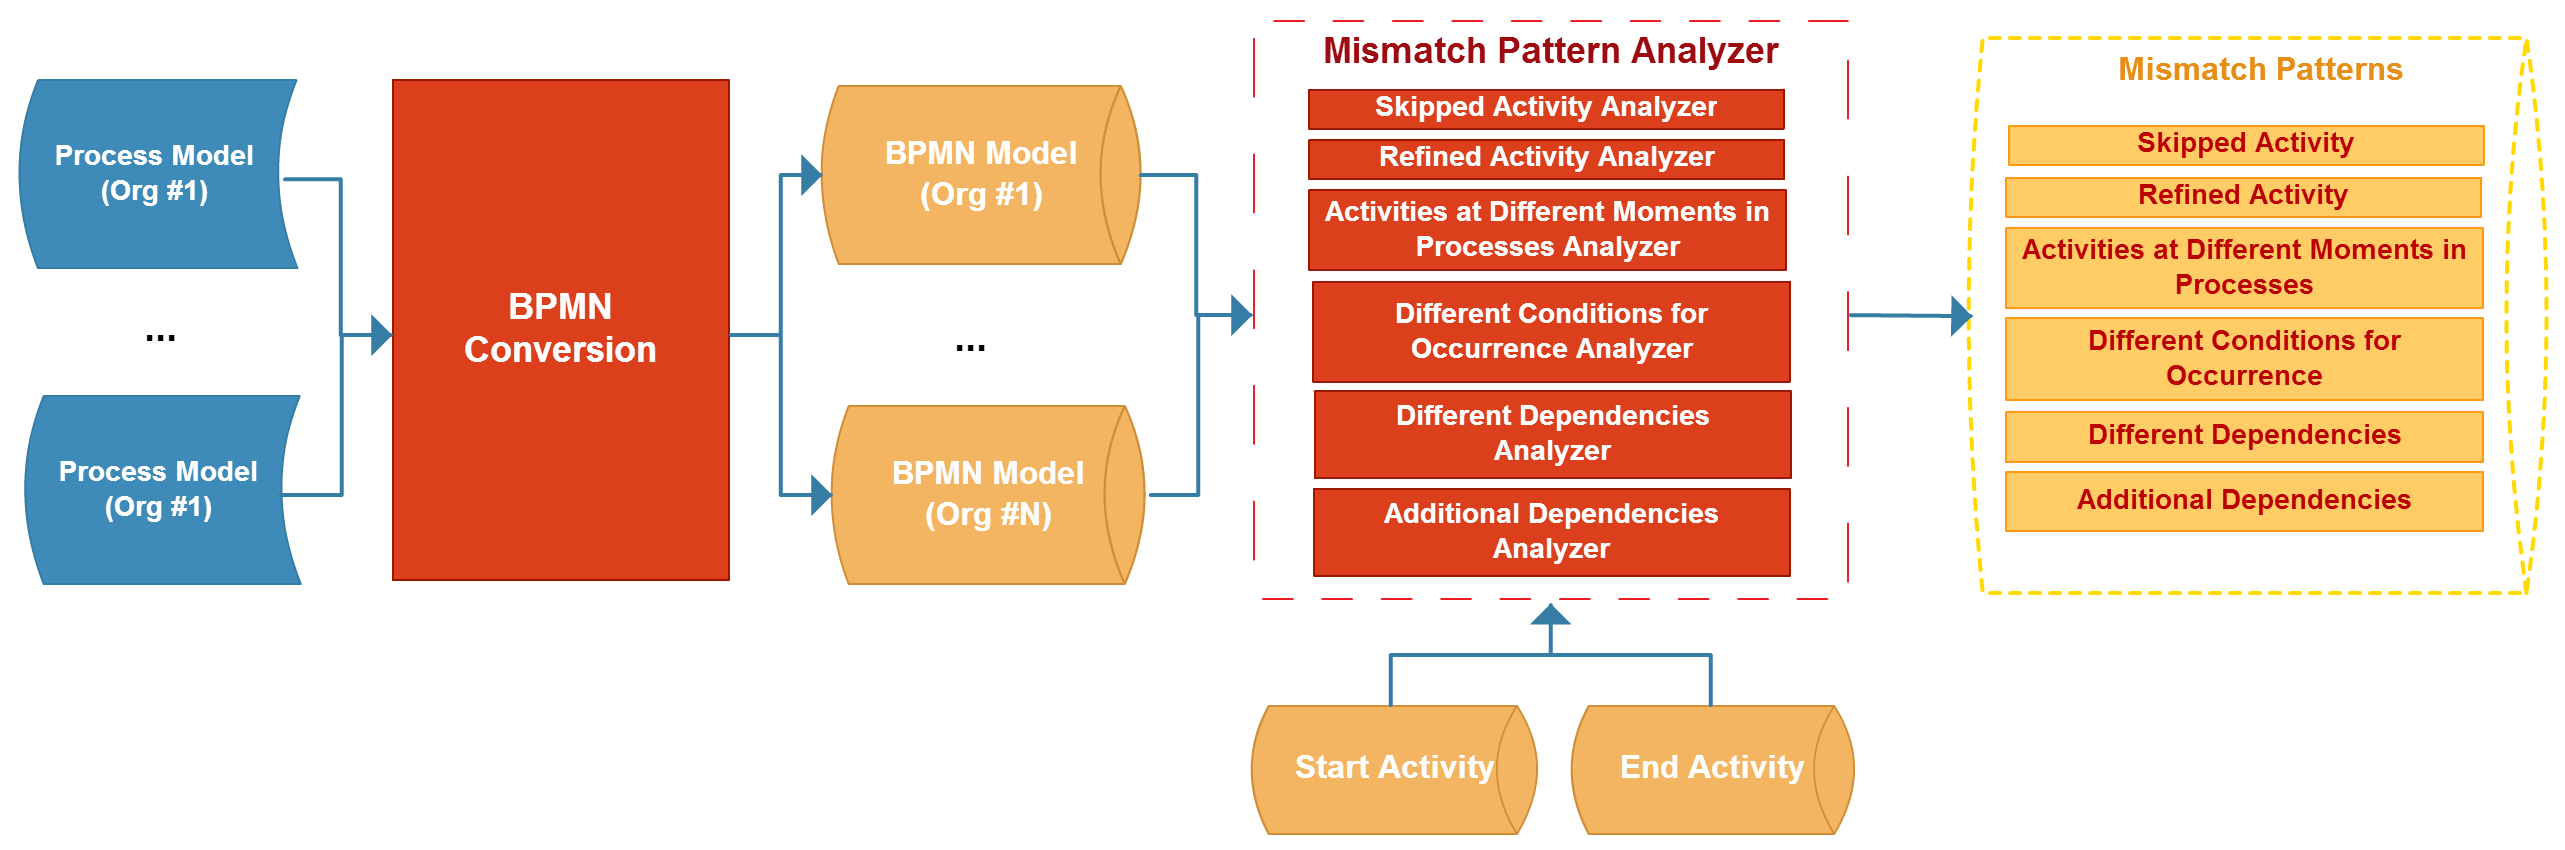
\includegraphics[width=\textwidth]{4_methodology/mismatch-pattern-analysis-blackbox}
  \caption{Mismatch Pattern Analysis Stage as Black-box}
  \label{fig:mismatch-pattern-analysis-blackbox}
\end{figure}

\begin{algorithm}
\DontPrintSemicolon % Some LaTeX compilers require you to use \dontprintsemicolon instead 
\KwIn{$O_{1}$ first organization, $O_{2}$ second organization, $A_{start}$ starting activity, $A_{end}$ ending activity}
\KwOut{$MismatchPatterns$ a set of mismatch patterns}
$MismatchPatterns \leftarrow \{\}$ \;
$MismatchPatterns$ \leftarrow  SkippedActivityAnalyzer($O_{1}$,$A_{start}$,$A_{end}$) \;
$MismatchPatterns$ \leftarrow  RefinedActivityAnalyzer($O_{1}$,$O_{2}$,$A_{start}$,$A_{end}$) \;
$MismatchPatterns$ \leftarrow  DifferentMomentsAnalyzer($O_{1}$,$O_{2}$,$A_{start}$,$A_{end}$) \;
$MismatchPatterns$ \leftarrow  DifferentConditionsAnalyzer($O_{1}$,$O_{2}$,$A_{start}$,$A_{end}$) \;
$MismatchPatterns$ \leftarrow  DifferentDependencysAnalyzer($O_{1}$,$O_{2}$,$A_{start}$,$A_{end}$) \;
$MismatchPatterns$ \leftarrow  AdditionalDependencysAnalyzer($O_{1}$,$O_{2}$,$A_{start}$,$A_{end}$) \;
\Return{$MismatchPatterns$}\;
\caption{Mismatch Pattern Analysis}
\label{algo:mismatch}
\end{algorithm}

\section{Recommendation Generation}
\label{sec:recommendation-generation}
Recommendation generation stage in the methodology is the final and core stage where all information retrieved from event logs until now are utilized. Till this point, all event logs are used to mine process models of each organization and then these event logs are replayed on the process models to calculate performance indicators. Following these steps, the organizations are clustered based on their performance indicators and mismatches between their process models are listed. In this stage, clustering results, which are performance indicator vectors for each cluster will be used to generate recommendations for each cluster of organizations based on the differences between their mismatch patterns.

In this study, idea of recommendation is based on providing a set of mismatch patterns for each organization so that they can enhance their processes. These mismatch patterns are generated by comparing the process models of other organizations, particularly which are performing better in terms of their performance indicator values. In addition, clustering of organizations is undertaken generalize the way of identifying which organizations perform better in this environment. Recommendation idea and recommendation generation function is defined as following:
\theoremstyle{definition}
\begin{definition}
Recommendation is a tuple 

${Recommendation} = (O, A_{start}, A_{end}, Mismatch\ Patterns) $ where 
	\begin{enumerate}
	  \item $O$ is identifier for organization,
	  \item $A_{start}$ and $A_{end}$ are starting and ending activities in between the recommendations are checked,
	  \item $Mismatch\ Patterns$ is collection of mismatch patterns.
	\end{enumerate}
\end{definition}

\theoremstyle{definition}
\begin{definition}
Recommendation generation is a function that is \textit{RecGen(O, C, P)} and it returns a set of \textit{Recommendation} where
	\begin{enumerate}
	  \item $O$ is identifier for organization,
	  \item $C$ is \textit{Cluster Analysis Data} which is result of cluster analysis stage,
	  \item $P$ is \textit{Performance Threshold} which is a real number larger than or equal to 0.
	\end{enumerate}
\end{definition}

Algorithm of recommendation generation function is based on the idea of checking other clusters for a significant change in performance indicators, where significance is defined by the threshold provided by user. After finding significant difference, all organizations in other clusters are checked against mismatch patterns with the starting and ending activities defined in performance indicators. With this constraining, only mismatches which are located between the activities that causes high level of difference in performance indicators are analyzed. This approach is formalized in Algorithm~\ref{algo:recgen}.
 \begin{algorithm}
\DontPrintSemicolon % Some LaTeX compilers require you to use \dontprintsemicolon instead 
\KwIn{$O$ organization, $C$ Cluster Analysis Data, $P$ performance difference threshold}
\KwOut{$Recommendations$ a set of recommendations}
$Recommendations \leftarrow \{\}$ \;
$i \leftarrow C(Assignments(O))$ \;
\For{$Centroid \in C(Cluster Centroids_{i})$} { 
	\For{$Centroid' \in C(Cluster Centroids_{j}))\ i\neq j$} { 
		\If{$Centroid(A_{start}) = Centroid'(A_{start}) \& Centroid(A_{end}) = Centroid'(A_{end})$} {
			\If{ ($\left |  Centroid(Value) -  Centroid'(Value)\right | \div Centroid(Value)) \geq P$  } {
				$A_{start} \leftarrow Centroid(A_{start})$ \;
				$A_{end} \leftarrow Centroid(A_{end})$ \;
				$MismatchPatterns \leftarrow \{\}$ \;
		 		\For{$O' \in C(Assignments(j))$} {
					$MismatchPatterns$ \leftarrow  Mismatch Pattern Analysis($O$,$O'$,$A_{start}$,$A_{end}$) \;
				}
				$Recommendations$ \leftarrow  Recommendation($O$,$A_{start}$,$A_{end}$, $MismatchPatterns$) \;
			}
		}
	}
}
\Return{$Recommendations$} \;
\caption{Recommendation Generation}
\label{algo:recgen}
\end{algorithm}

This stage of methodology can be visualized as gathering inputs of mismatch patterns data and cluster analysis data in Figure~\ref{fig:recommendation-generation-blackox}. In addition, a performance difference threshold is gathered from the user to specify how much difference between clusters is necessary to check for mismatch patterns and generate recommendations. This stage generates recommendation data for each organization which contains a set of mismatch patterns.
\begin{figure}
  \centering
  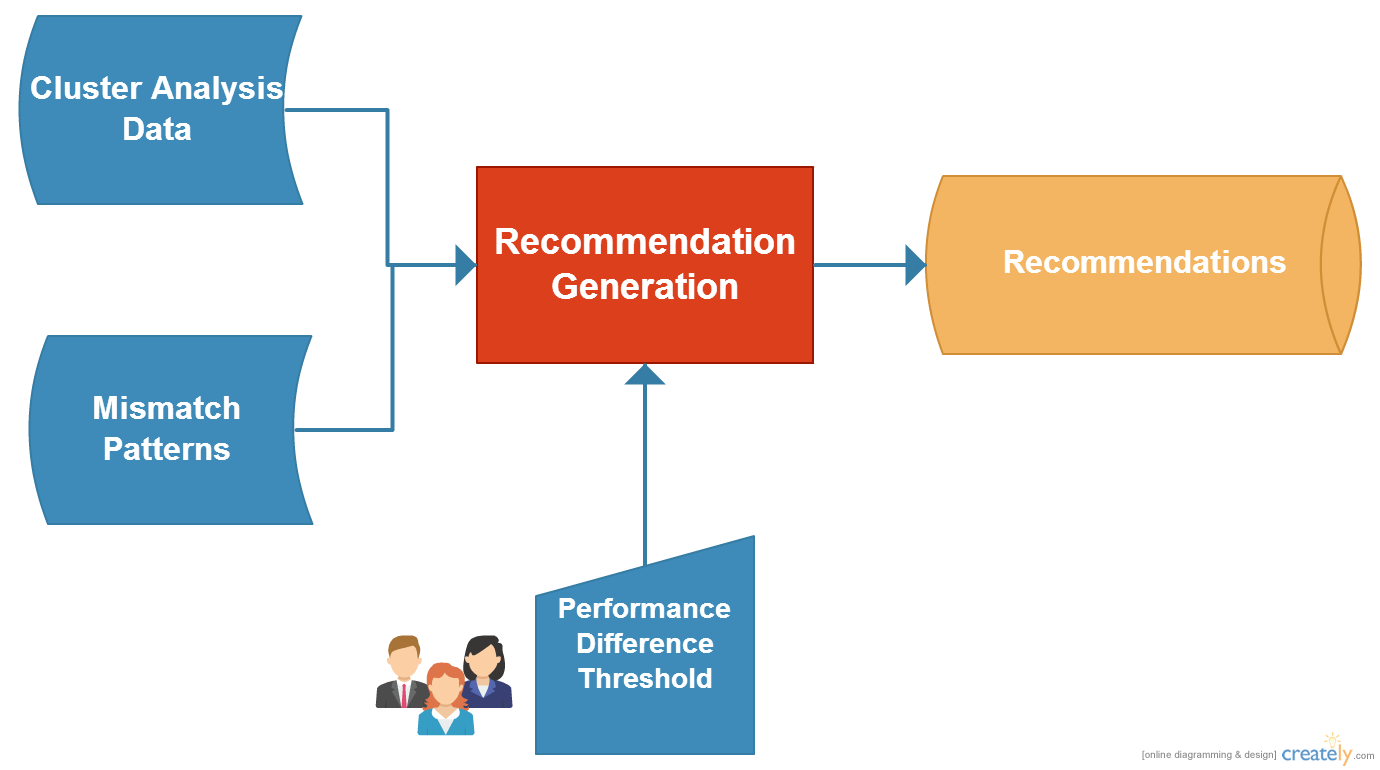
\includegraphics[width=\textwidth]{4_methodology/recommendation-generation-blackbox}
  \caption{Recommendation Generation Stage as Black-box}
  \label{fig:recommendation-generation-blackox}
\end{figure}

\section{Implementation in ProM Framework}
\label{sec:implementation}
\todo{WRITE}

Methodology of this thesis study is implemented in ProM Framework \cite{verbeek2010prom}, which is an extensible framework that supports a wide variety of process mining techniques in the form of plugins. Approach of this thesis study is implemented with its each stage as a standalone plugin that enables extensions for further studies. Developed set of plugins are packaged with the name of \textit{CrossOrgProcMin} and it is available in the latest version of ProM release. 

PROM öv

Implementation details are presented from two perspectives in this section. Firstly, software architecture of methodology implementation will be explained with the relationships and dependencies with other plug-ins and ProM framework. Then, user experience perspective will be presented to show how an end user of this methodology can provide inputs, make analysis and gather results. 

\subsection{Software Architecture}
\label{subsec:architecture}
Approach of this study is divided into standalone stages where inputs and outputs between them are defined strictly. With the help of this understanding, each stage is developed as a standalone plugin in ProM framework which can be called separately. For this aim, five plugins are developed which are visualized in Fig~XX to provide a high-level perspective. In addition, a set of utilities are developed to visualize and persistence of data in ProM environment. 

\begin{description}
  \item[Cross-Organizational Process Mining] is the core plugin which handles management and data flow between other plugins. It basically calls each other plugin and gathers outputs from them to proceed to next plugins. 
  \item[Process Miner Plugin] is the implementation of Section~\ref{sec:process-model-mining} where \textit{Inductive Miner} \cite{leemans2014discoveringinfrequent} package in the ProM environment is utilized. 
  \item[Automated Replayer Plugin] is developed to execute the approach in Section~\ref{subsec:replay-and-performance-summary} and it replays the event logs over process models with the minimum manual user input using the libraries in \textit{Peti Net Replayer} package \cite{adriansyah2011towards}. 
  \item[Cluster Analysis Plugin] is developed to cluster the organizations based on their performance indicators as presented in Section~\ref{subsec:performance-indicator-clustering} and this plugin uses WEKA libraries \cite{hall2009} which are external to the ProM environment. 
  \item[Mismatch Analysis Plugin] is developed to discover differences between the process models as explained in Section~\ref{sec:mismatch-pattern-analysis}. This plugin is developed from scratch since there is no implementation of mismatch patterns \cite{dijkman2007mismatch} in ProM framework.
  \item[Utilities] are developed to handle input and output data to the developed set of plugins. Import and export libraries are coded to enable data specific persistence in ProM framework for these plugins. Visualization libraries are developed to represent the recommendation output to the end user in ProM screens.
\end{description}   


\subsection{User Experience}
\label{subsec:architecture}
toplama olduğunu, user için gerekenleri bahset


\chapter{RESULTS AND DISCUSSIONS}
\label{chp:results-and-discussions}

In this chapter, methodology presented in this thesis study is applied on datasets and results are presented. Firstly, evaluation metrics are defined for each stage of methodology to evaluate performance of the approach. Following this, methodology is applied on two datasets and results are explained with discussions.

\section{Evaluation Metrics}
\label{sec:evaluation-metrics}
Approach in this study is an aggregation of various methods and they are significantly different from each other in their mathematical background. Therefore, instead of a global evaluation metric for the complete methodology, each stage will be evaluated within its evaluation metrics. Since these stages are executed sequentially, it is important for each stage to perform enough well to yield a successful outcome. In this section, evaluation metrics for each stage will be presented and they will be used to determine the success of methodology on experiments.

\subsection{Process Model Mining}
\label{subsec:process-model-mining-eval}
Process model mining stage takes input as event logs of organizations and creates process models using process mining algorithms, namely \textit{Inductive Miner} \cite{leemans2014discoveringinfrequent}. Performance of this stage can be measured by the conformance of the process models to the the event logs. Four competing quality criteria are defined in \cite{van2011process} and they are \textit{fitness}, \textit{simplicity}, \textit{precision} and \textit{generalization}. Fitness is based on the idea of being able to replay event log over process model whereas precision focuses not underfitting the event log. Simplicity idea is based on the fact that the simplest model is the best model, on the other hand generalization supports not overfitting the event logs. These four competing criteria are mathematically defined in \cite{rozinat2008conformance} and grouped into two dimensions for analysis purposes:

\begin{description}
  \item[Fitness] Event log and the process model should \textit{fit} to each other, in other words process model should be able to parse the event log. 
  \item[Appropriateness] Since \textit{fitness} does not provide information about the meaningfulness of process models, this dimension is defined. Two notions comprise this idea; \textit{Structural Appropriateness} considers the simplicity whereas \textit{Behavioral Appropriateness} analyzes balance between overfitting and underfitting.
\end{description}

In this thesis study, process model mining stage will be evaluated by the \textit{Fitness} and \textit{Appropriateness} of the mined process models for each organization. In ProM  It is expected to have higher \textit{fitness}, closer to 1, and a high level of appropriateness to continue to the next stages with the high quality process models. While evaluating, \textit{fitness} will be more dominant since \textit{appropriateness} without \textit{fitness} means less.
%	conformance plugin'i çağır, filtre ekranında var, 
%	structural olanı elle hesapla -> http://wwwis.win.tue.nl/~wvdaalst/publications/p436.pdf pg21
\subsection{Performance Indicator Analysis}
\label{subsec:performance-indicator-analysis-eval}
Performance indicator analysis stage consists of two parts as replaying event logs over process models and clustering organizations based on the performance indicators. In the replay phase, main operation is to \textit{align} \cite{van2012replaying} event logs and process models. This alignment is the based on the idea of finding the optimal alignment where total cost of \textit{move on process model} and \textit{move on event log} are minimized. Since there is no baseline information for alignment costs of organizational logs, total cost information will be used together with the process model mining evaluation metrics. In other words, for the event logs and process models with known conformance metrics, total cost of alignments will create a secondary check if there are any problems related to replaying events over process models. It is expected to have less total cost of alignment for the organizations with higher conformance since it is easy to align event logs and processes with high superior fitness values.
% Şu pluginle bak: Check compliance using conformance checking ->
For the second stage of performance indicator analysis, there is a need to evaluate performance of clustering organizations. In this stage, organizations are clustered  based on their performance indicator values that are calculated over replaying. Since there is no labeled data in the context of this thesis study, any cross-validation techniques could not be applied and thus internal evaluation metrics are exploited. As mentioned in the Section~\ref{subsec:performance-indicator-clustering}, within SSE values between clusters are plotted to the end user to select an appropriate number of clusters. It is expected that within SSE values decreases as number of clusters increases; however, number of clusters should be selected without causing overfitting.
% wekadan gelen within sse 

\subsection{Mismatch Pattern Analysis}
\label{subsec:mismatch-pattern-analysis-eval}
Mismatch pattern analysis stage aims to find differences between the process models of different organizations. In this thesis study mismatch patterns defined in \cite{dijkman2007mismatch} are mathematically defined and analyzers are developed to locate these patterns. At the time of this study, it is known to be first to use mismatch patterns in a generic method, therefore evaluation is based on comparing with well-defined prior similarity metrics.

Structural similarity between process models is presented in \cite{dijkman2011similarity} by the \textit{graph-edit distance} notion. In graph theory, \textit{graph-edit distance} is the minimum number of \textit{graph-edit operations} necessary to get one from graph to another. In the process mining field, \textit{graph-edit operations} are simply node addition, deletion or substitution. In the study \cite{dijkman2011similarity}, both \textit{graph-edit distance} and \textit{graph-edit similarity} definitions are provided with their mathematical background. In this study, mismatch pattern analysis stage is evaluated by comparing the number of mismatch patterns and the \textit{graph-edit similarity} of process models. Without any performance indicator clustering, it is expected to have larger number of mismatch patterns when the similarity between process models is low. This will ensure the performance and suitability using mismatch pattern analysis instead in the methodology.
 % BartHompes paketi ile ikili ikili çalıştır- run
\subsection{Recommendation Generation}
\label{subsec:recommendation-generation-eval}
In the recommendation generation stage, set of mismatch patterns are presented to the end user based on the selected organization and performance difference threshold. This stage aims to list whole mismatch patterns that can cause the other organizations perform better than a difference threshold. Idea of using performance threshold should be evaluated in this stage with its responsiveness. In other words, it is expected that this stage will help the end user to focus on the most important performance improvements for the organization analyzed. Therefore, different threshold values will be tried to check how many mismatch patterns are generated for organizations and how they could be used for focused analysis. In addition, quality and applicability of the recommendations should be analyzed and this requires a high level of knowledge starting from the collecting event logs in the organizations. This knowledge should include know-how about process changes, domain knowledge about the field of organizations' activity and structural attributions of the organizations.

\section{Dataset Selection}
\label{sec:dataset-selection}
Cross-organizational mining aims to find cross-correlation of workflows and activities in different organizations and this yields the necessity of organizations that do the same main activity with a comparable process flows. In business life, this includes aligning the tasks from different organizations with different business needs, priorities and organizational structures and culture. Considering these characteristics, there are few dataset available in the literature that are well-structured, documented and valuable. In this thesis study, one synthetic and one real-life event log datasets  are presented and used in the following sections to evaluate the performance of the proposed methodology.

\begin{description}
  \item[Loan Application Process \cite{loan-app-data}] This synthetically created dataset consists of event log variants of a simple loan application in a financial institute. In summary, a customer fills a form and starts a request over website and it starts the different approaches of variants in different organizations that ends with notifying the customer about the acceptance of application. This dataset includes artificial event logs of 4 variants where each variant includes different sets of approaches such as parallelism, choices and sequential tasks. These event logs are used to test different approaches of discovering a configurable process model from a collection of event logs in study \cite{buijs2014flexible}.
  \item[Environmental Permit Application Process \cite{coselog-data}] This dataset originates from the "Configurable Services for Local Governments (CoSeLoG)" project \cite{van2011business} which investigates the similarities and dissimilarities between several processes of different municipalities in the Netherlands.  Dataset contains the records of the execution of the receiving phase of the building permit application process in 5 municipalities, which are comparable since activity labels in the different event logs refer to the same activities performed in the five municipalities. This data set is also mentioned in the literature as \textit{"Processing applications for building and/or environmental permits (Wet Algemene Bepalingen omgevingsrecht (WABO) in Dutch)"}.

  When the organizations that have similar processes are considered, municipalities are one of the prominent candidates. In Netherlands there are more than 400 municipalities and they offer between 400 and 500 different products and services with their own processes. Unlike corporations, municipalities have the advantage that they can seek for collaboration since they are not direct competitions \cite{buijs2012towards} and this advantage makes them valuable for cross-organizational analysis. CoSeLoG research project aims to develop a shared business process management system within a shared Software-as-a-Service environment using the commonalities between the processes of municipalities \cite{buijs2014flexible}. In the scope of CoSeLoG research, five different processes of municipalities are analyzed and at the time of this thesis study only \textit{Environmental Permit Application Process} dataset is publicly shared in the literature.
\end{description}

\section{Loan Application Process}
\label{sec:loan-app-process}
In this section, methodology proposed in this thesis study will be applied on the \textit{Loan Application Process} dataset \cite{loan-app-data} and evaluation results will be presented. Statistical information about this dataset is presented in Table~\ref{table:loan-app-process-summary}.
%\caption{Statistical summary of Loan Application Process Dataset}
%\label{table:loan-app-process-summary}
\begin{table}[]
\centering
\caption{Statistical summary of Loan Application Process dataset}
\label{table:loan-app-process-summary}
\begin{tabular}{@{}lccc@{}}
\toprule
                  & {\bf Cases} & {\bf Events} & {\bf Percentage} \\ \midrule
{\bf Variant \#1} & 100         & 590          & 24 \%            \\ \midrule
{\bf Variant \#2} & 70          & 420          & 17 \%            \\ \midrule
{\bf Variant \#3} & 200         & 800          & 33 \%            \\ \midrule
{\bf Variant \#4} & 105         & 630          & 26 \%            \\ \midrule
{\bf Total}       & {\bf 475}   & {\bf 2440}   & {\bf }           \\ \bottomrule
\end{tabular}
\end{table}

As shown in Table~\ref{table:loan-app-process-summary}, total of 475 cases and 2440 events included in this dataset with a fairly even distribution between variants. In the following sections, these variants will be used as organizational logs and the methodology presented in this thesis study will be applied.

\subsection{Methodology Stages}
\label{sec:loan-app-methodology}
In \textit{Process Model Mining} stage, variants of the dataset are used as organizational event logs and they are used to mine process models. Since dataset is synthetically generated, noise threshold in \textit{Inductive Miner} is set to 0 and perfect log fitness is ensured. Appropriateness and fitness evaluation metrics are summarized in Table~\ref{table:loan-app-process-process-model-mining} and it can be seen that each event log is successful in terms of representing reality and being appropriate as a process model. Especially for the variants other than Variant #1, there is a perfect fitness and appropriateness as it is expected from a  synthetically generated dataset without noise. In addition, process models for each event log is visualized in Figure~\ref{fig:loan-application-process-models}.

%\caption{Process Model Mining Evaluation of Loan Application Process Dataset}
%\label{table:loan-app-process-process-model-mining}
\begin{table}[]
\centering
\caption{Process Model Mining Evaluation of Loan Application Process Dataset}
\label{table:loan-app-process-process-model-mining}
\begin{tabular}{lcccc}
\hline
 & {\bf Fitness} & {\bf \begin{tabular}[c]{@{}c@{}}Structural\\ Appropriateness\end{tabular}} & {\bf \begin{tabular}[c]{@{}c@{}}Behavioral\\ Appropriateness\end{tabular}} & {\bf \begin{tabular}[c]{@{}c@{}}Average\\ Appropriateness\end{tabular}} \\ \hline
{\bf Variant \#1} & 100 \% & 70 \% & 98,5 \% & 84,25 \% \\ \hline
{\bf Variant \#2} & 100 \% & 100 \% & 100 \% & 100 \% \\ \hline
{\bf Variant \#3} & 100 \% & 100 \% & 100 \% & 100 \% \\ \hline
{\bf Variant \#4} & 100 \% & 100 \% & 98,2 \% & 99,1 \% \\ \hline
{\bf Average} & {\bf 100 \%} & {\bf 92,5 \%} & {\bf 99,7 \%} & {\bf 96,06 \%} \\ \hline
\end{tabular}
\end{table}
 
\begin{figure}
\centering
\begin{subfigure}{.4\textwidth}
  \centering
  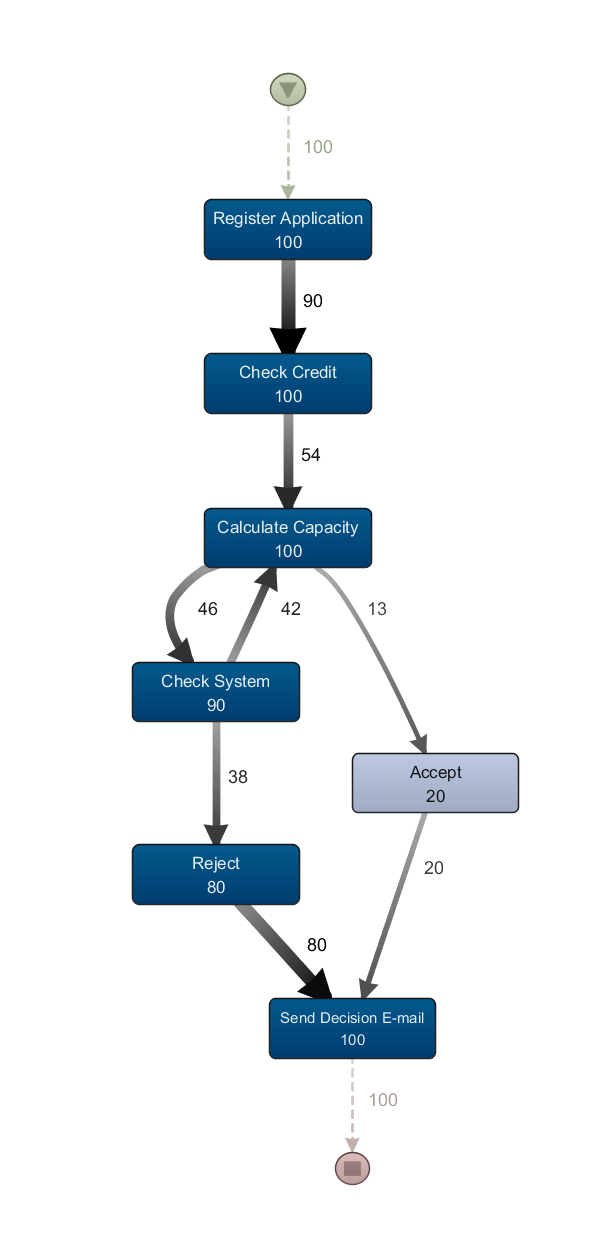
\includegraphics[width=.8\linewidth]{5_results_discussions/loan-application-process/ETM_Configuration1}
  \caption{Variant #1}
  \label{fig:loan-application-process-models-1}
\end{subfigure}%
\begin{subfigure}{.4\textwidth}
  \centering
  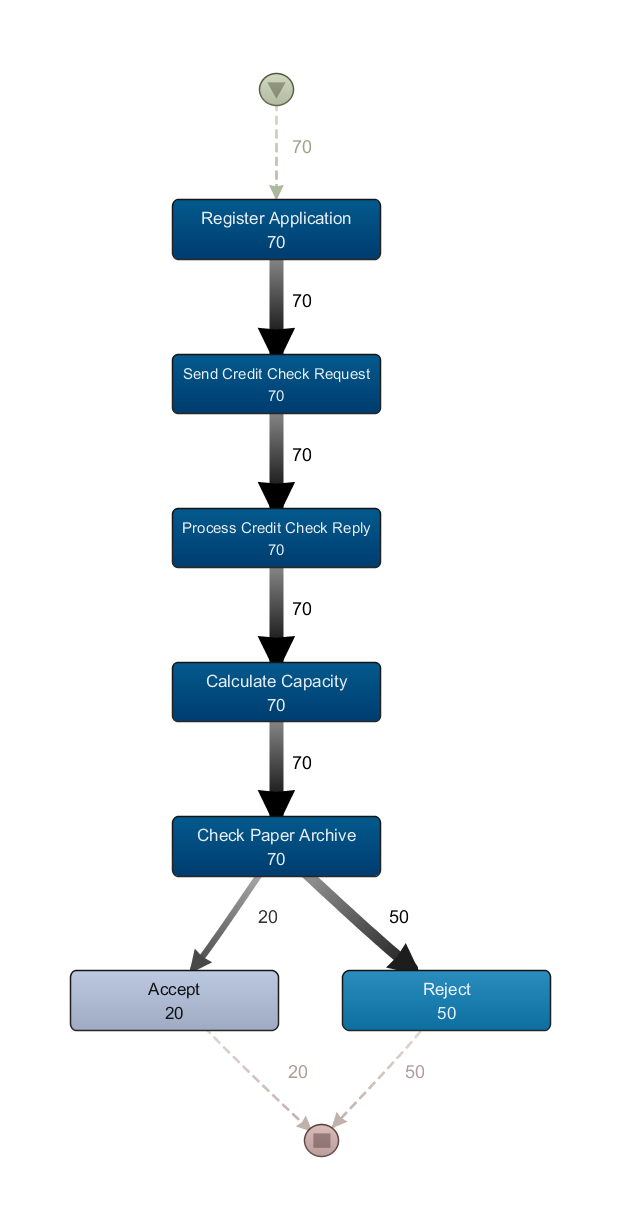
\includegraphics[width=.8\linewidth]{5_results_discussions/loan-application-process/ETM_Configuration2}
  \caption{Variant #2}
  \label{fig:loan-application-process-models-2}
\end{subfigure} \\
\begin{subfigure}{.4\textwidth}
  \centering
  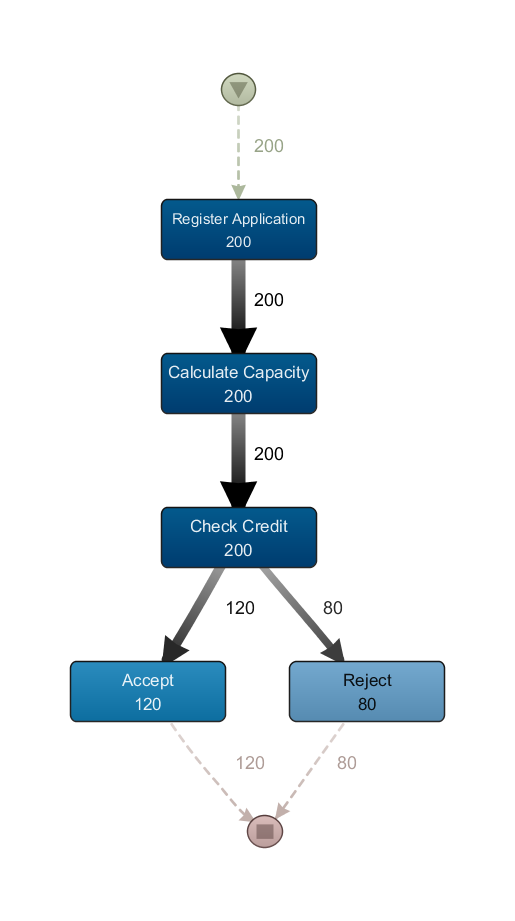
\includegraphics[width=.8\linewidth]{5_results_discussions/loan-application-process/ETM_Configuration3}
  \caption{Variant #3}
  \label{fig:loan-application-process-models-3}
\end{subfigure}%
\begin{subfigure}{.4\textwidth}
  \centering
  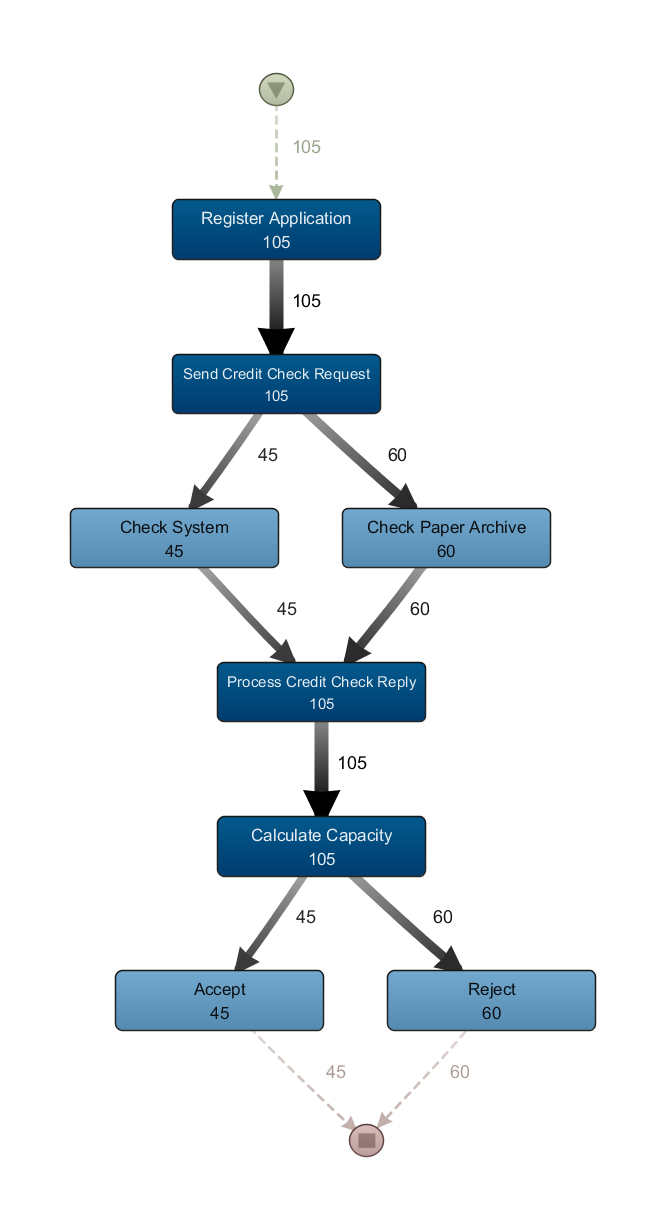
\includegraphics[width=.8\linewidth]{5_results_discussions/loan-application-process/ETM_Configuration4}
  \caption{Variant #4}
  \label{fig:loan-application-process-models-4}
\end{subfigure}
\caption{Process models of Loan Application Process dataset}
\label{fig:loan-application-process-models}
\end{figure} 

In \textit{Performance Indicator Analysis} stage, firstly event logs are replayed over process models and performance indicators are calculated. For replaying step, alignment costs should be checked with respect to process model mining evaluation metrics; however, since all fitness values of variants are 100 \% in Table~\ref{table:loan-app-process-process-model-mining}, alignment costs are 0 for all variants in this dataset. This ensures that event logs are successfully replayed over process models and performance indicators are calculated. With these performance indicators, organizational logs will be clustered

In \textit{Mismatch Pattern Analysis} stage, number of mismatch patterns are analyzed with the \textit{graph-edit similarity} between each two organization. As the similarity between process models decreases our method spots more mismatch patterns for most of the variant comparisons and it ensures that the developed mismatch pattern analyzers work as expected for this dataset. Correlation between \textit{graph-edit similarity} and number of mismatch patterns are plotted in Figure~\ref{fig:loan-mismatch-pattern-analysis-results}.

\begin{figure}
	\centering
	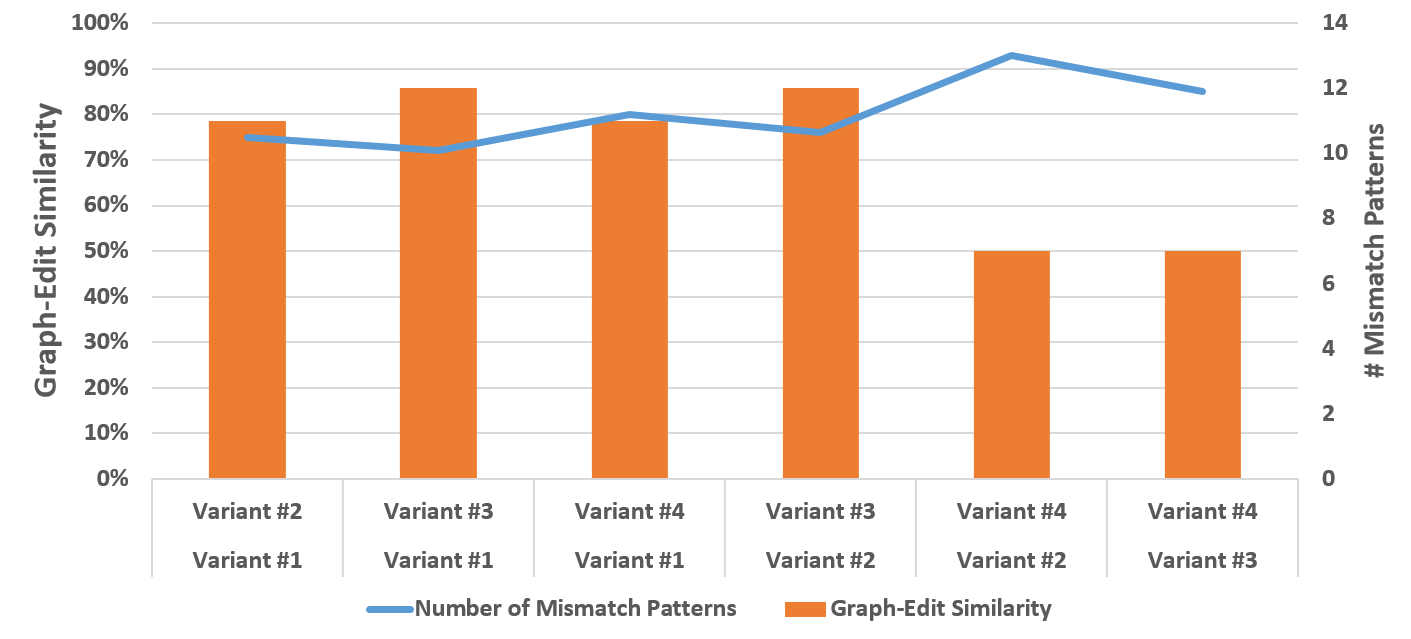
\includegraphics[width=\textwidth]{5_results_discussions/loan-application-process/mismatch-pattern-analysis-results}
	\caption{Mismatch Patterns vs. Graph-Edit Similarity for Loan Application Process Variants}
  \label{fig:loan-mismatch-pattern-analysis-results}
\end{figure}

When the mismatch patterns are analyzed according to their types as plotted in Figure , Skipped Activity and Activities at Different Moments patterns are spotted mostly and no Different Conditions for Occurrence or Additional Dependencies patterns are spotted. Considering the small amount of this dataset, these numbers and distribution can be counted as acceptable.

\begin{figure}
	\centering
	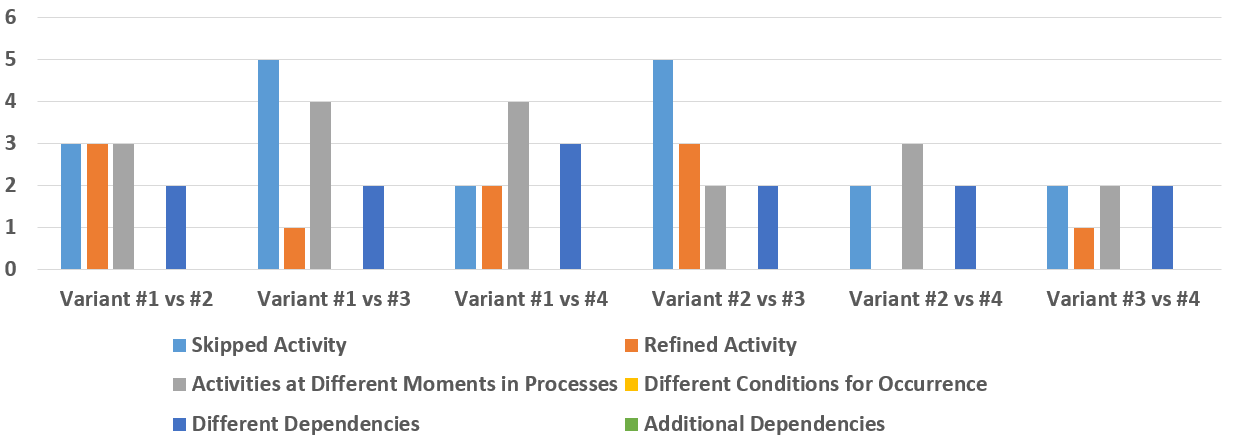
\includegraphics[width=\textwidth]{5_results_discussions/loan-application-process/mismatch-pattern-types}
	\caption{Mismatch Pattern Types for Loan Application Process Variants}
  \label{fig:loan-mismatch-pattern-types}
\end{figure}
 

% recommendation generation analysis
% burada da cluster'lar arası mismatch pattern sayısını farklı thresholdlar için dene


\subsection{Results}
\label{sec:loan-app-results}
% burada yukarıdaki çıkanları özetle + çıkan önerilerden bir tanesini falan çizerek anlat

\section{Environmental Permit Application Process}
\label{sec:environmental-permit-application-process}
 
* Event log statistics
* Methodology Stages
* Results

\section{Discussions}
\label{sec:discussions}
\chapter{CONCLUSION AND FUTURE WORK}
\label{chp:conclusion-and-future-work}

\section{Conclusion}

In this thesis study, a new approach is proposed and tested for generating recommendations using cross-organizational process mining for process performance improvement. Cross-organizational process mining is applied with the idea of unsupervised learning where predictor variables related to performances of organizations are used in an environment where processes are executed on several organizations. Results show that it is possible to use cross-organizational process mining and mismatch patterns for performance improvement recommendations. Process mining is a large-spectrum field where different set of activities and approaches are gathered together to discover, monitor and improve processes. In this thesis study, a four-stage solution is presented and their performances are explained.

Process mining stage mines the process models of different organizations and it is shown that a generic, noise-capable process mining method can create process models with high fitness and appropriateness values. This indicates that mining process models of different organizations under a generic method can yield comparable and appropriate process models. Success of this stage directly affects the quality of calculated performance indicators since they are collected through the replay of event logs over process models.

Performance indicator analysis stage in the methodology clusters the organizations based on their performance indicators and internal evaluation metrics show that it is suitable to cluster organizations based on how well they are operating. Although there are studies that clusters organizations based on their process models for structural analysis \cite{greco2005mining}, this approach showed that organizations can be clustered based on their performance indicators.

Mismatch analysis stage in this thesis has the aim of spotting differences between processes of organizations and it is known to be the first implementation of mismatch patterns \cite{dijkman2007mismatch}. When the results of this stage is checked against well-established similarity metrics in the literature, it can be concluded that mismatch pattern finding can be used when there is a need for spotting differences in similar processes. 

Recommendation generation stage collects the generated and extracted information in all prior stages to list what the organizations can learn from other organizations which perform better. In order to define performing better, different thresholds are checked for each organization and resulting recommendations show that clustering organizations based on performance indicators and then checking mismatch patterns significantly helps user to focus on the differences with a potential performance improvement. In addition, quality of recommendations in business usefulness is tried to be explained with example outputs and these examples show that the approach yields recommendations difficult to spot manually and visually, which are also potential causes of performance improvement.

In addition, proposed methodology is developed as extensible and configurable set of plugins in ProM framework \cite{verbeek2010prom} and published as open-source. This makes the methodology open to include new process mining methods, mismatch patterns and clustering approaches as well as testing with different datasets.

\section{Future Work}

For the approach proposed in this thesis study, the following issues can be listed as pointers to future work:
\begin{itemize}
	\item In the process mining stage, instead of \textit{Inductive Miner}, different techniques can be used which can mine complex process models with higher appropriateness levels while keeping the current high fitness values.
	\item In the performance indicator analysis stage, new indicators can be defined based on the business environment, event log attributes and user needs. For instance, personnel and resource allocation indicators can be included as well as cost dimension.
	\item For mismatch pattern analysis, new and business oriented mismatch patterns can be included in the analysis. In addition analyzers can fail when there are loops in the process models in current implementations, therefore more robust implementations for process models with loops can be developed in the future.
	\item For the generated recommendation, their quality for business environment are not assessed within the scope of this thesis. However, when any feedback from a domain expert or BPM people is provided, the learning approach can be converted to semi-supervised learning from unsupervised learning.
	\item For ProM implementation of this study, currently user selects an organization to list recommendations; in the future user might be able to select area of interest as well as starting and ending points visually on a process model. 
\end{itemize}


\bibliographystyle{plain}
%
% References in Bibtex format goes into below indicated file with .bib extension
\bibliography{7_references/references}
% You can use full name of authors, however most likely some of the Bibtex entries you will find, will use abbreviated first names
% If you don't want to correct each of them by hand, you can use abbreviated style for all of the references

\appendix
\chapter{APPENDIX}

\section{Methodology Steps}
\label{sec:appendix-methodology-steps}
\begin{figure}
	\centering
	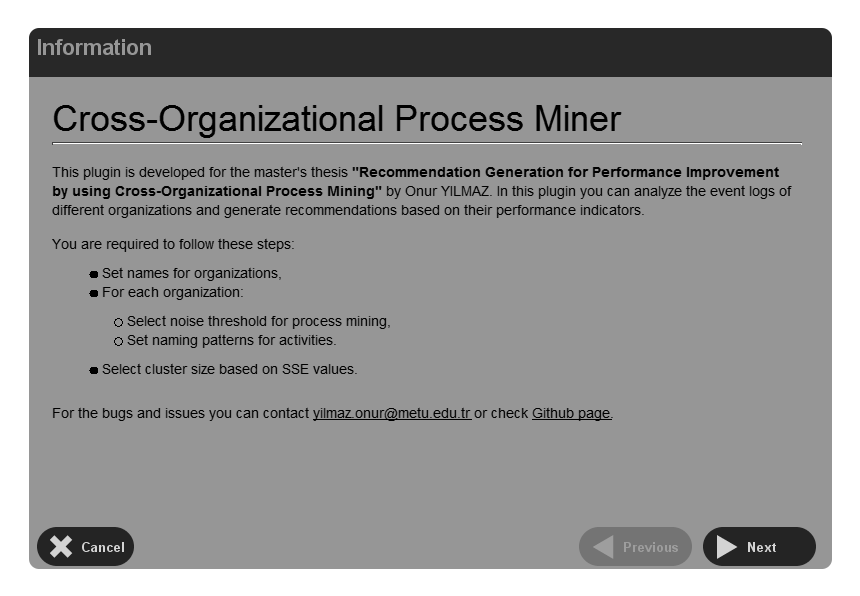
\includegraphics[width=\textwidth]{8_appendix/information-screen}
	\caption{Information Screen of Cross-Organizational Process Miner Plugin}
	\label{fig:information-screen}
\end{figure}
asd

\begin{figure}
	\centering
	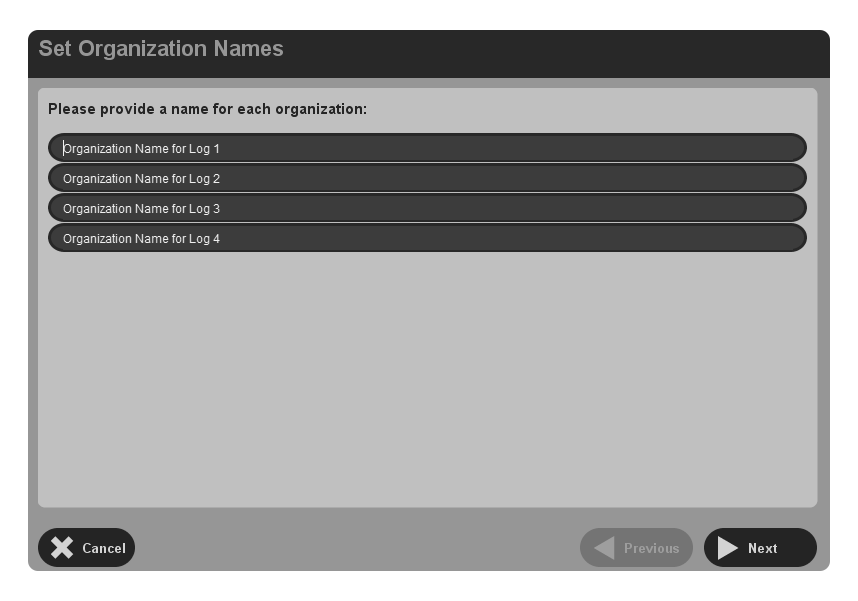
\includegraphics[width=\textwidth]{8_appendix/organization-name-screen}
	\caption{Organization Naming Screen of Cross-Organizational Process Miner Plugin}
  \label{fig:organization-name-screen}
\end{figure}

\begin{figure}
	\centering
	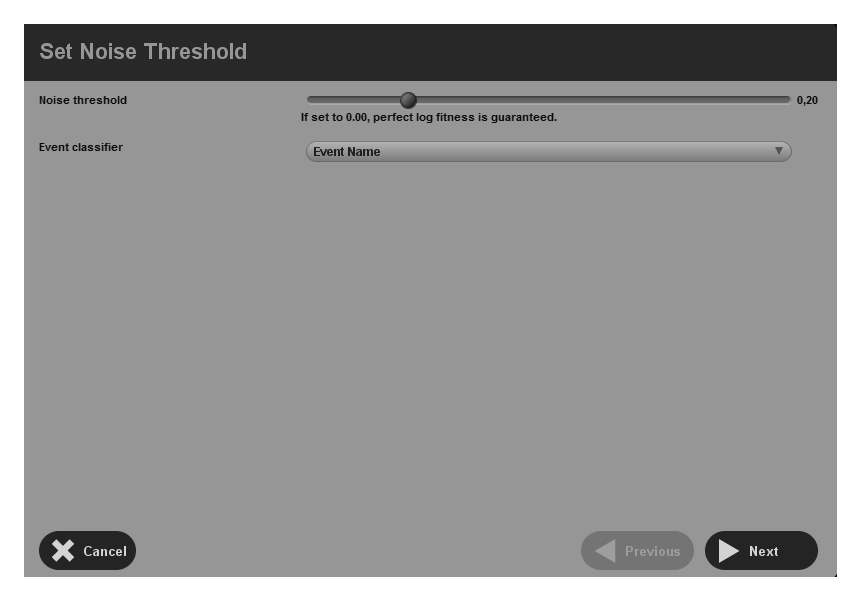
\includegraphics[width=\textwidth]{8_appendix/proc-miner-threshold-screen}
	\caption{Process Miner Screen of Cross-Organizational Process Miner Plugin}
  \label{fig:proc-miner-threshold-screen}
\end{figure}

\begin{figure}
	\centering
	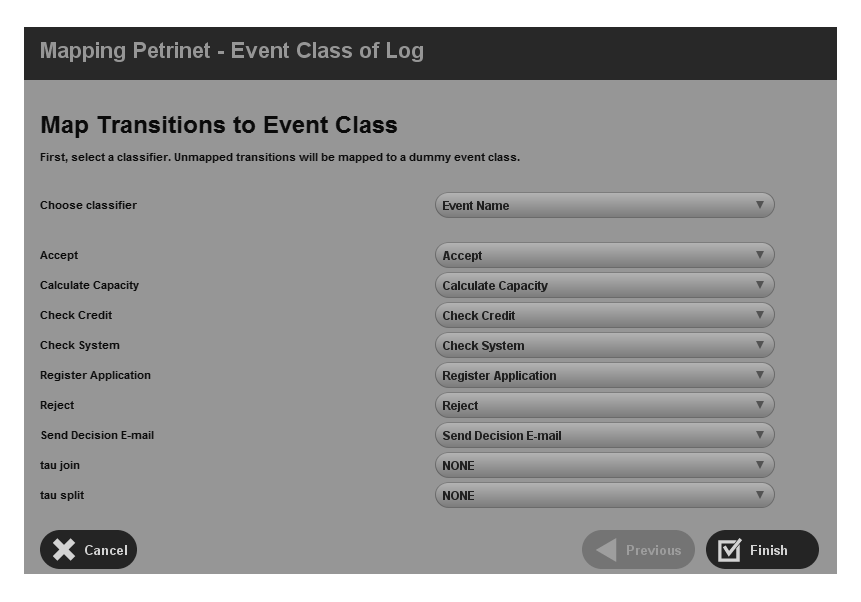
\includegraphics[width=\textwidth]{8_appendix/automated-replayer-screen}
	\caption{Automated Replayer Screen of Cross-Organizational Process Miner Plugin}
  \label{fig:automated-replayer-screen}
\end{figure}


%\chapter{Appendix Name}
%%%Appendix content goes here.
 
%
% If you are a Ph.D. Student you need to insert a CV at the end of you thesis
% Check vita.tex for a simple CV template in Latex
% \curriculumvitae
\label{chapter:vita}

\section*{\uppercase{Personal Information}}

\textbf{Surname, Name: } Surname, Name\\
\textbf{Nationality:} Turkish (TC) \\
\textbf{Date and Place of Birth:} dd.mm.yyyy, City\\
\textbf{Marital Status:} Single \\
\textbf{Phone:} 0 312 0000000 \\
\textbf{Fax:} 0 312 0000000 \\

\section*{\uppercase{Education}}

\begin{tabular}{lll}
\textbf{Degree} & \textbf{Institution} & \textbf{Year of Graduation} \\
M.S. & M.S. Institute & M.S. Year \\
B.S. & B.S. Institute & B.S. Year \\
High School & High School Name & High School Graduating Year
\end{tabular}

\section*{\uppercase{Professional Experience}}

\begin{tabular}{lll}
\textbf{Year} & \textbf{Place} & \textbf{Enrollment} \\
Duration 1 & Institute/Company 1 & Role/Position/Experience 1 \\
Duration 2 & Institute/Company 2 & Role/Position/Experience 2 
\end{tabular}

\section*{\uppercase{Publications}}
\subsection*{International Conference Publications}
Your publications goes here. Do not try to use Bibtex, since Bibtex builds a single bibliography
database for the document.

\end{document}
